\chapter{Prediction}\label{ch:prediction}

{
    \section{Introduction}
     {
      The ability to predict the impact of transformation on urban environments is a critical aspect of city-planning. Unlike other industries, urban interventions cannot sustain trial-and-error or A-B testing, thus requiring high degree of confidence and well established risk-aversion mechanisms \cite{doi:10.1080/14649357.2015.1127994, banerjee2011companion}. Urban forecasting could be generally described via a two axes graph: (i) the prediction time-frame, and (ii) the social - physical spectrum (see Figure \eqref{fig:predictions_axis})
      .\newline
      For example, predicting the shadows casted by a new building, is directly correlated to the building's context, as well as to its bulk and shape. Evidently, as long as the earth spins around the sun, the results of shadow modeling should be consistent, and the model describing this phenomena could be reused indefinitely.
      On the other end, a predictive model of potential human interaction in a public plaza, would share much less consistency across time and space. This model would heavily rely on social and cultural aspects, as well as physical attributes of the urban realm, such as the plaza's shape, or its proximity to certain amenities. This class of predictions, which focuses on spatial, temporal, and social aspects, is clearly harder to construct, validate, and reuse, but can make significant impact on decision-making. As reviewed in Section \eqref{subsec:andorra-data-observatory-mobility}, this class of predictions is slowly becoming mainstream in urban processes, with the growing access to location, activity, and behavioral data, as well as new computation and modeling techniques \cite{jiang2017activity, Calabrese2014, Batty2013, moro2021mobility}.
     }

    \begin{figure}[!htb]
        \begin{center}
            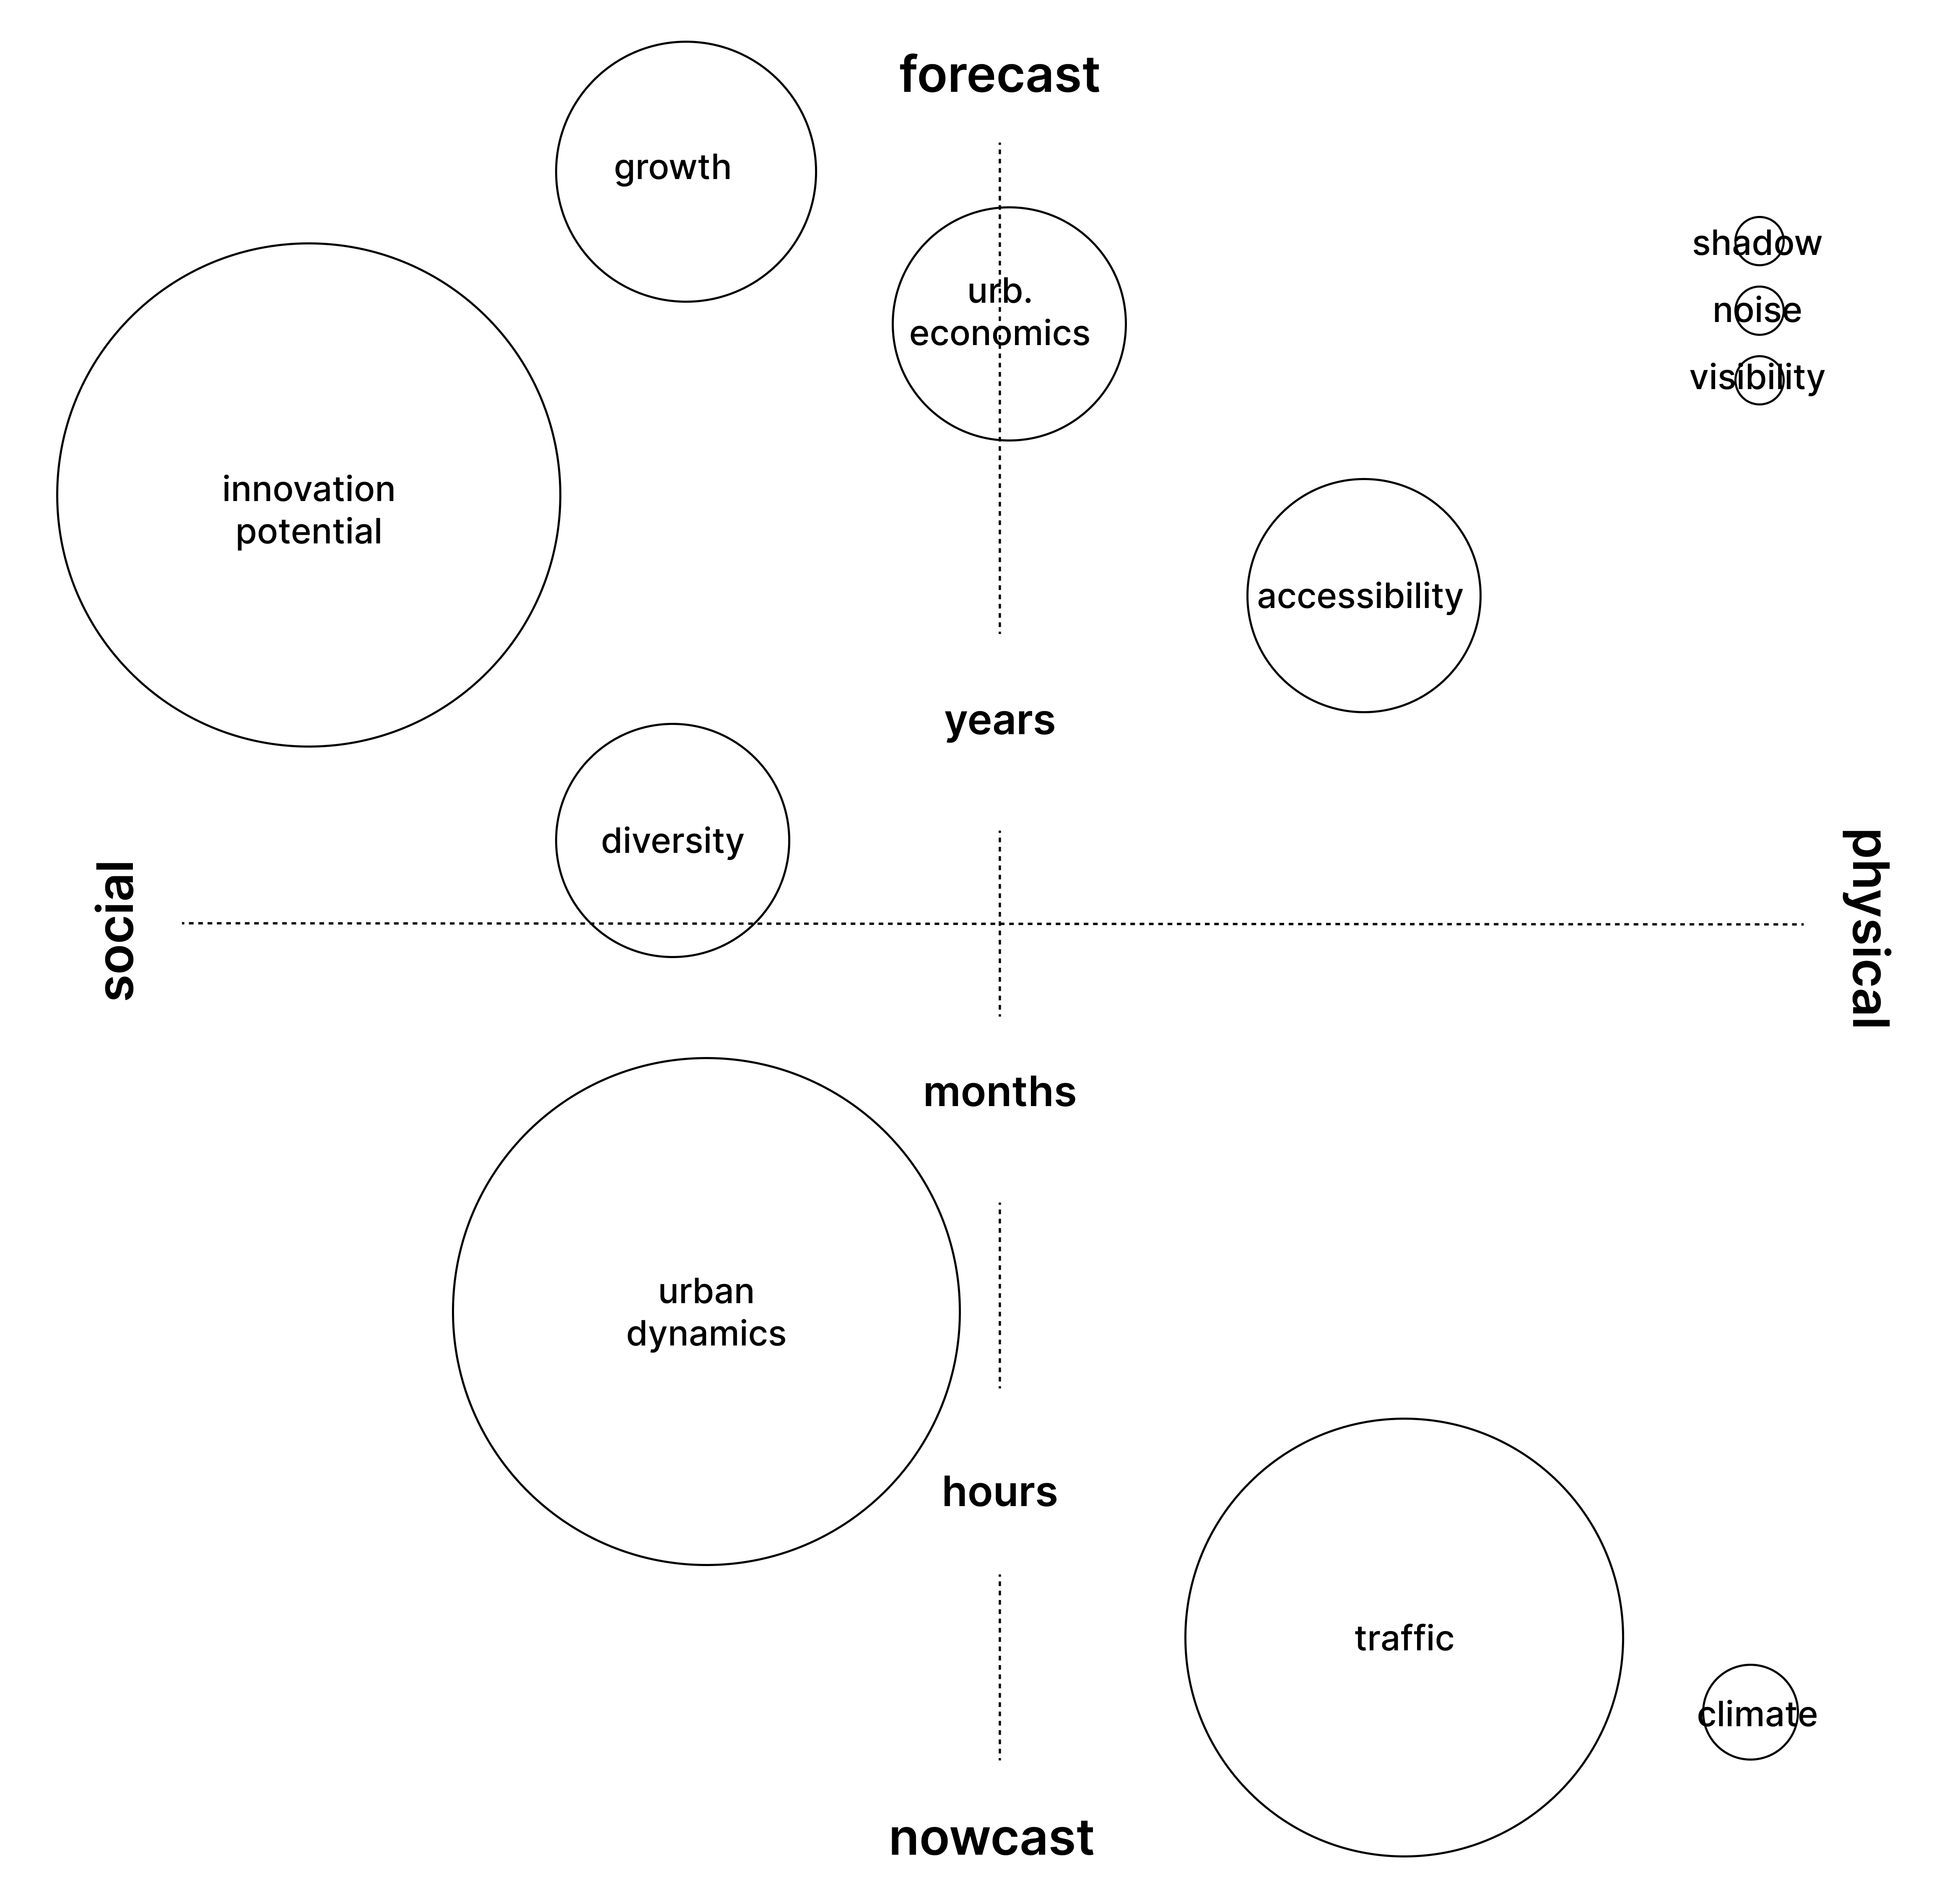
\includegraphics[width=0.8\textwidth]{chapters/prediction/figures/predictions_chart.png}
        \end{center}
        \caption{The landscape of urban predictions. This is a visual clustering of the high-dimensionality of different urban models. The horizontal axis represents the degree of `concreteness' for each prediction (i.e., where does this metric seats between the less tangible and more physical?). The vertical axis depicts the longevity of the prediction (i.e., how far into the future can this metric be predicted?). The size of the dots hints to the estimated span of the prediction across the two axes; For example, predicting shadows is more concrete and longer-term than predicting human behavioral patterns.}
        \label{fig:predictions_axis}
    \end{figure}

    \section{CityScope Prediction: Case Studies}
     {
      The previous chapter discussed ways by which CityScope supports predictions of long-term, physical aspects of the built environment. These included assessments ranging from Gross Floor Area, storm-water runoff, and building energy, to more complex models, such as noise propagation (see \eqref{ch:transformation}).
      \newline
      This chapter focuses on a class of predictive models at the intersection of human behavior and the built environment. These projects combine geo-spatial attributes (such as urban form, POIs, and street network graphs), socio-behavioral properties (interpreted from high-resolution telecom data), and other discrete datasets.
      In the \textit{CityScope MoCho} project (see Section \eqref{sec:modeChoices}), mobility mode choices were simulated using a city-wide synthetic population. Static data, such as census and National Household Travel Surveys (NHTS) were used to construct simulated profiles of daily commuters and assign them to home-work and 3rd places anchors. By interpreting plausible trips from socio-demographic data, the model forecasts how small scale changes to land-use can affect large scale mobility behaviors.
      \newline
      A simulated urban population can also help to understand emergence and agglomeration patterns. In CityScope \textit{Volpe}, \textit{Andorra} and \textit{Champs-Élysées} (see \eqref{sec:and_abm}, \eqref{sec:cityscope_volpe}, \cite{ChampsEl64:online}) Agent Based Models are used to simulate trips, `collision potential', and mode-choice changes caused by urban-design transformations. A similar approach was taken in the \textit{Hamburg Port-City Model} \cite{lopez2019testing}, in which an ABM was built to predicate changes to tourist activity in transit hubs and the city's port, given minor adjustments to queuing and boarding. A different type of predictions involves the usage of data-driven models to forecast implicit and `subtle' changes in urban environments. The \textit{DeepScope} \eqref{sec:deepscope} project uses Generative Adversarial Networks (GAN) to `imagine' streetscapes of future urban developments\footnote{Upcoming work in this domain will correlate behavioral patterns and user-experiences of urban streets, with the visual aspects of new urban development.}.
      \newline
      The rest of this chapter will describe how these implicit models were implemented in several CityScope projects.
     }

    %%%%%%%%%%%%%%%%%%%%%%%%%%%%%%%%%%%%%%%%%%% 
    \section{MoCho}\label{sec:cityscope-mocho}
{
    \subsection{Introduction}
    {
        Understanding the impact of city-planning on mobility habits of urban dwellers is fundamental to well functioning cities. Nevertheless, it is challenging to predict, communicate, and demonstrate the correlation between minor urban interventions and metropolitan scale mobility mode-choices (MC). CityScope `MoCho' is a real-time MC modeling and prediction module that simulates MC of individuals in a metro region, in response to small-scale urban-design transformation. The prediction models consider individual characteristics and attributes of available alternatives, and are calibrated using survey data. To explore MoCho MC predictions, users interact with the CityScope TUI which triggers new MC predictions, alongside their impacts based on land-use, density or spatial proximity. As a case-study, MoCho has been developed to simulate MC for the Boston metro area, focusing on a 14 acres development site in Kendall Sq. (see Section \eqref{appendix:playground}). The choice model was fitted and the parameters showed significant associations with a range of explanatory variables, including travel times, residential and employment densities, as well as personal attributes like age, gender, education-level and home-ownership.
    }



    \begin{figure}[!htb]
        \centering
        \includegraphics[width=.7\linewidth]{chapters/prediction/mocho/figures/mocho2.png}
        \caption{
            MoCho and CityScope TUI. Interaction results are computed and visualized on both vertical (metro-scale) and horizontal (parcel-scale) planes. A TUI slider (bottom left corner) allows density and building-height iteration for the land-use type used as the slider handle.
        }
        \label{fig:mocho_tui}
    \end{figure}

    \subsection{Motivation}
    {
        The individual choices urban dwellers make about their mobility and transportation behavior have profound impacts on their own lives, as well as on society as a whole. Motorized transportation leads to negative external impacts such as carbon emissions and air pollution, whereas active mode-choices such as walking and cycling improve the physical and mental health of travelers \cite{doorley2015quantifying, mueller2015health}. Urban-planning can influence these mobility choices and their societal impacts by organizing spatial land-uses and infrastructure to encourage short trips using active modes \cite{handy2002built, saelens2003environmental}. Statistical learning methods have been used successfully both in research and in practice to predict the mode-choices of travellers in response to urban interventions \cite{ben1999discrete, wardman2007factors, habib2009investigation, buehler2016bikeway}.
        \newline
        Making predictions through statistical models, generally involves the combination of various computing platforms\footnote{Most commonly in R \cite{hasan2014fast}, Stata \cite{gu2013fitting}, specialized transportation modeling software such as SimMobility \cite{adnan2016simmobility} or Python and GIS plugins.}. These may carry steep learning curves, require specialized skills, and feature limited capabilities for real-time interaction \cite{ben-joseph2001}. In this study, a CityScope instance was devised to overcome these challenges using a combination of real-time statistical models with an interactive, real-time user interface.
    }

    \subsection{Data and Modeling} \label{sec:mocho-models-data}

    {
        MoCho makes use of publicly available datasets which cover major urban areas in the US; This ensures that the methodology presented here can be replicated for the vast majority of American cities. The main data resources used are specified in Table \ref{tab:mocho-dataSources}.

        \begin{table*}[!tb]
            \centering
            \begin{adjustbox}{width=\textwidth}
                \begin{tabular}{ll}
                    \hline
                    \textbf{Resource}                              & \textbf{Description}                                                               \\
                    \hline
                    Public Use Microdata Sample (PUMS)             & Individual person and household level survey data for the USA                      \\
                    American Community Survey (ACS)                & Aggregated demographic data for administrative zones in the USA                    \\
                    OpenStreetMap (OSM)                            & An open-source editable map of the world \cite{haklay2008openstreetmap}            \\
                    Open Source Routing Machine (OSRM)             & An API which provides routing information using OSM data \cite{huber2016calculate} \\
                    Open Trip Planner (OTP)                        & A server which computes multi-modal transport itineraries \cite{OTP}               \\
                    Census Transportation Planning Products (CTPP) & A special tabulation of the ACS data for commuting characteristics                 \\
                    \hline
                \end{tabular}
            \end{adjustbox}
            \caption{Data resources used for US cities in CityScope MoCho}
            \label{tab:mocho-dataSources}
        \end{table*}

        These data sources are used to generate a synthetic population and to calibrate a model which could predict their mobility behaviors in response to changes, such as new residential or commercial development. The modeling can be described in four steps: (i) Population synthesis; (ii) Home and job location choices; (iii) Transportation mode-choice; and (iv) Impact assessment. Each of these steps is outlined below.
    }

    \subsubsection{Population Synthesis}
    {
        Mobility behaviors can be analyzed using two main approaches: (i) An aggregate approach, which divides the area into zones and predicts aggregates inter-zonal flows, or (ii) A disaggregate approach, which recognizes that urban mobility patterns are the result of many decisions made by individuals. The disaggregate approaches directly explain why an individual makes a choice given their circumstances, and therefore they are better able to predict how those choices may change in different circumstances \cite{koppelman2006self}. Due to privacy and data availability constraints, it is generally not practical to make predictions with respect to real population. Instead, it is common practice to use population synthesis techniques in order to produce a \textit{Synthetic Population}, and to make predictions with respect to these individuals. The methods take individual household-level demographic profiles and zonal aggregate demographic data, and allocate the individual records to zones in order to create the synthetic population. Some common techniques include Iterative Proportional Fitting \cite{beckman1996creating, guo2007population}, convex optimization \cite{vovsha2015new}, and Bayesian methods \cite{sun2015bayesian}.
        \newline
        The PUMS survey data used here includes the home Public Use Microdata Area (PUMA) and place-of-work PUMA for each respondent, where each PUMA corresponds to a set of census tracts. In order to model commuting trips at a tract-to-tract level, the population synthesis process needs to allocate each individual to a home and work census tract pair. A simple Bayesian method is utilized for this purpose, using the origin-destination flows from the CTPP data as well as aggregate demographic data from the ACS. PUMS individuals with attributes $A$, home PUMA $H$ and work PUMA $POW$ are assigned to an origin-destination (O-D) pair $w_{ij}$ according to the probability calculated with equation \eqref{mocho-eq-bayes}.

        \begin{equation}\label{mocho-eq-bayes}
            P(w_{ij}|A)\propto\delta_{ij}\prod_{a \in A}P(a|w_{ij})P(w_{ij})
            \\
            \quad where
            \\
            \quad
            \delta_{ij}=
            \begin{cases}
                1, & \text{if}\ H\subset i \text{ and } POW\subset j \\
                0, & \text{otherwise}
            \end{cases}
        \end{equation}

        The prior probabilities $P(a|w\_{ij})$ and $P(w\_{ij})$ may be obtained from the ACS aggregate demographic data and the CTPP O-D data.
    }

    \subsubsection{Home and Employment Location Choices}
    {
        MoCho aims to simulate the changes in home and work locations in response to amended land-use, density and spatial organization. It was assumed that when a residential or employment unit appears in a census tract, new residents or workers also appear. The number of new people is determined by the density of the unit; some demographic attributes, such as income or job sector, may be determined by the unit type. It is also assumed that the conditional probability distribution of the new residents' demographic attributes and work locations, is similar to that of the existing residents of that same tract, conditional on the known attributes. Therefore, the new resident can be simulated by cloning a randomly sampled person with the same home location tract and attributes from the synthetic population. A similar process is used to assign home locations to new workers; This location choice can be expected to be accurate for small changes to the land-uses and densities in a district but for more substantial changes, a more sophisticated model may be required.
    }

    \subsubsection{Mode-Choices}\label{sec:modeChoices}

    {
        The choice of transportation mode for each synthetic individual's commute should be predicted in response to each intervention. The mode-choices (MC) are modelled using a logit-based discrete choice model\footnote{Discrete choice models has been used extensively by researchers and practitioners in modeling of decisions including home location, work location and mode of transportation. An advantage of discrete choice models over other classification models is that their estimated parameters have economic interpretations; This means that the final model results can be easily understood by practitioners \cite{train2009discrete}.}. Discrete choice models assume that individual decision-makers select the alternative which maximizes their utility from their available options.
        \newline
        The utility is composed of a systematic component and a stochastic component: The systematic portion of the utility is (i) an additive function of attributes of the decision maker, (ii) attributes of the alternative, and (iii) interactions between both. This stochastic component is needed because in reality, two people with the same measured attributes may take different decisions when faced with similar alternatives. This component is typically assumed to be Gumbel distributed due to computational advantages and this leads to the logit formulation. These models can be defined by the following expressions \cite{koppelman2006self}:

        \begin{equation}\label{dcm}
            %   \begin{aligned}
            U(X_i, S_t)\geq U(X_j, S_t) \forall j \in C
            \quad \text{and}\quad
            U_{it}=V_{it} + \epsilon_{it}
            \quad \text{and}\quad
            V_{it}=V(S_t)+V(X_i)+V(S_t,X_i)
            %   \end{aligned}
        \end{equation}

        where $C$ is the choice set, $i$ is the alternative chosen by decision maker $t$,  $U_{it}$ is the true utility of alternative $i$ to decision maker $t$, $X_i$ are the attributes of option $i$, $S_t$ are the attributes of person t, $V$ is the systematic utility and $\epsilon$ is the stochastic utility.
        \newline
        The parameters of the logit model must be calibrated with individual-level stated-choice or revealed-choice data. For MoCho, individual observations from the PUMS data could be used for this calibration. The PUMS survey data contains 12 different options for MC but for the purpose of this work, this list is simplified to 4 major modes: car, bicycle, walk and public transportation modes. The explanatory variables considered for inclusion in the model include person attributes from the PUMS data (such as: age, income, gender, education level and employment type), attributes of the home and workplace census tracts from the ACS data, and the estimated travel times and costs for each mode and each trip. The travel times for each census tract pair were estimated by querying the OpenStreetMap API (for walking, cycling and driving times) and Open Trip Planner (for public transit travel times) \cite{OTP}. The PUMS data and ACS data contain hundreds of variables and so some exploratory analysis and feature engineering needs to be done to create a list of candidate features prior to model fitting. Once the features have been selected, the coefficients of each features can be estimated by maximum likelihood estimation, in this case using the python library `pylogit'.
    }


    \begin{figure}[!htb]
        \centering
        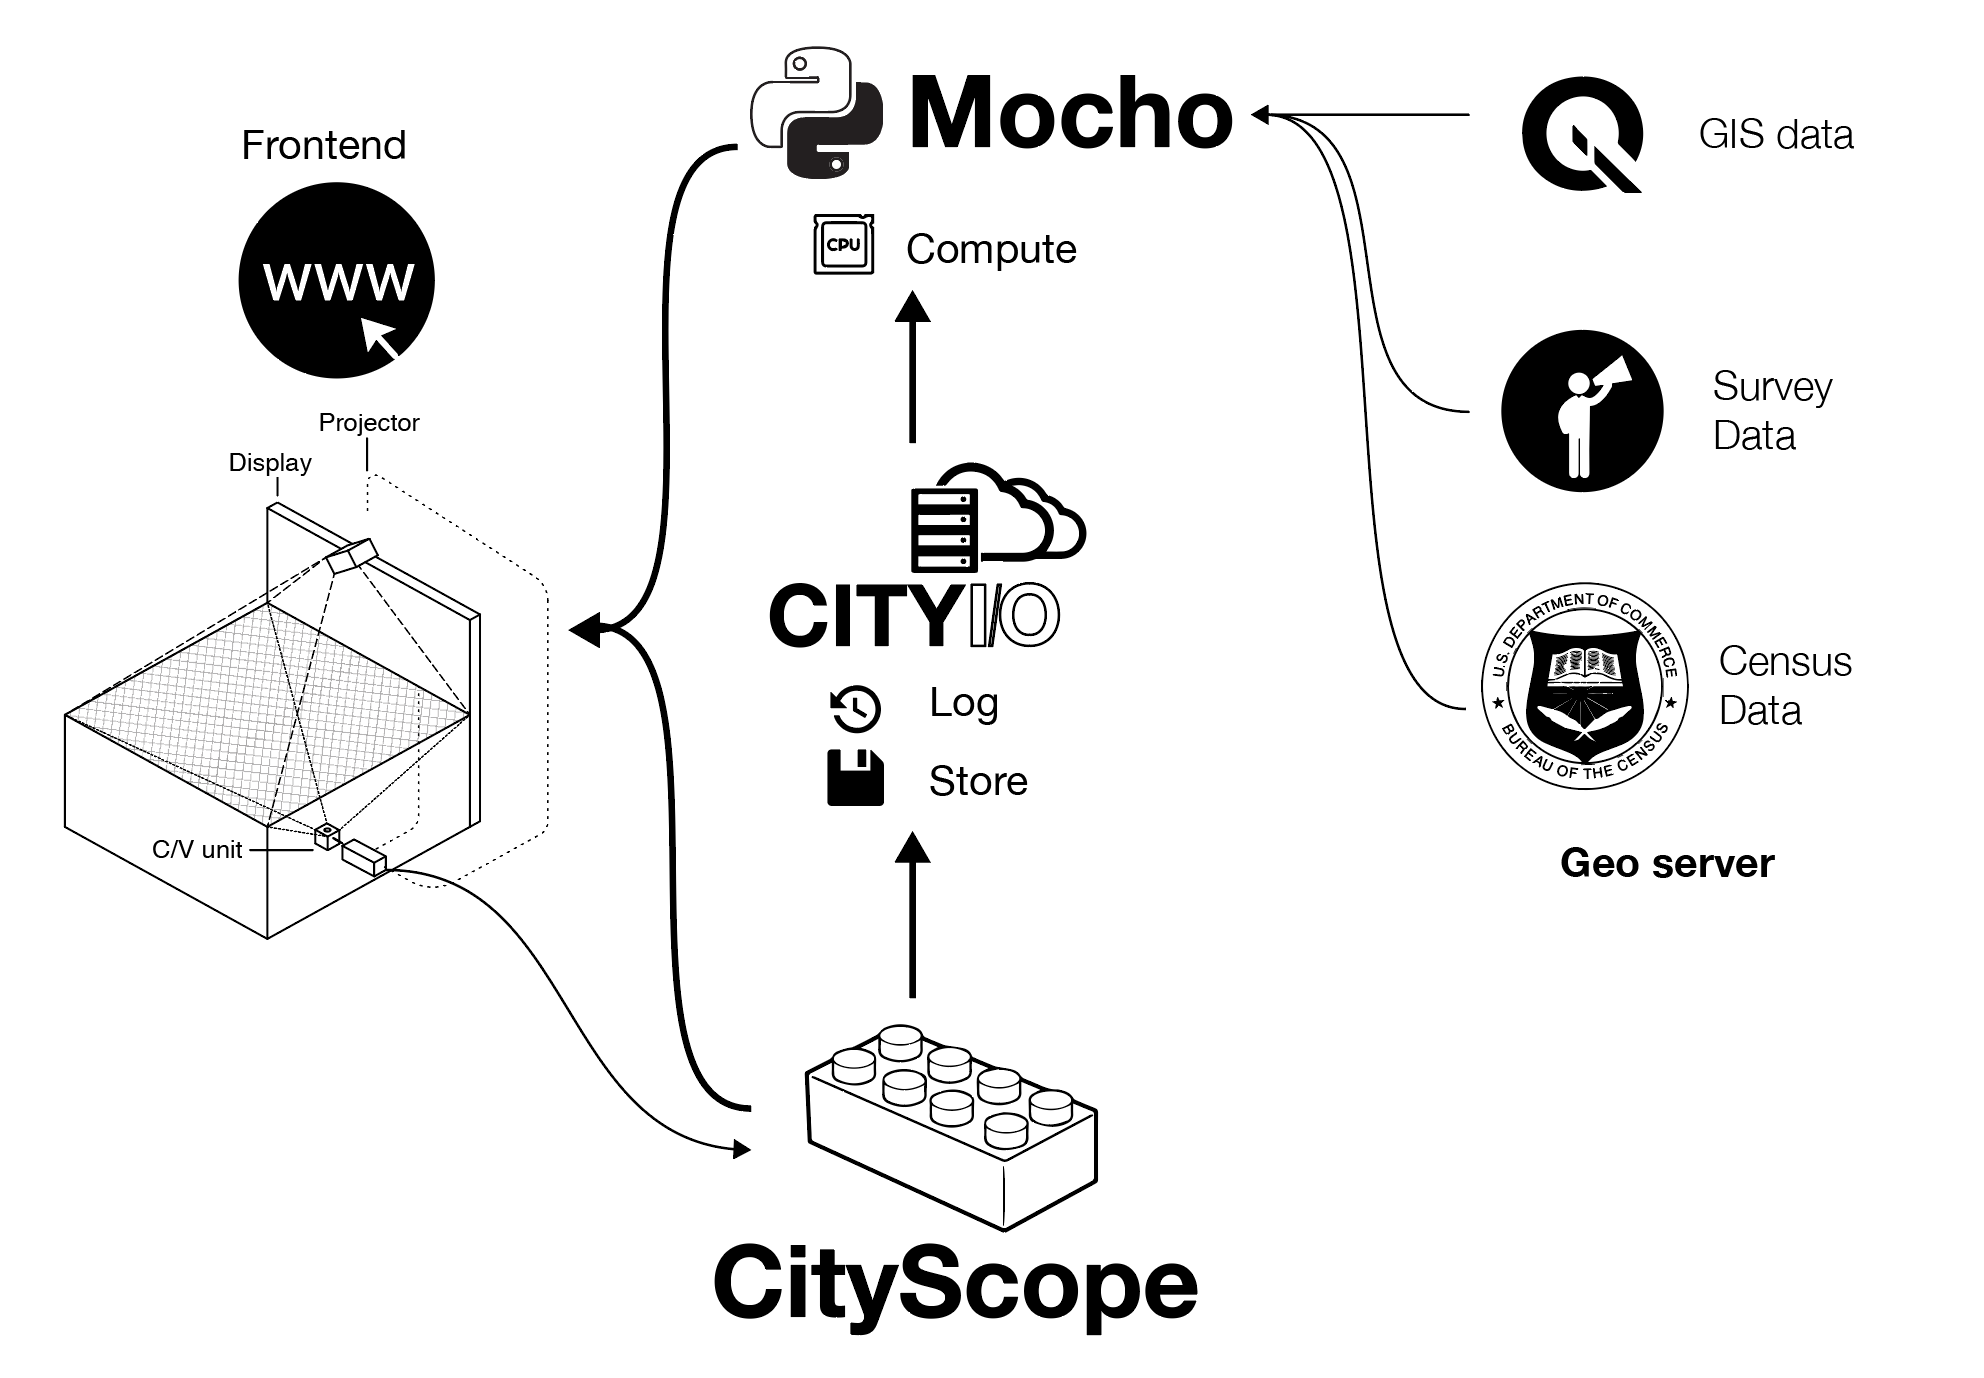
\includegraphics[width=.75\linewidth]{chapters/prediction/mocho/figures/mocho0.png}
        \caption{Software architecture. The CityScope table data is sent to cityIO from the tangible interface made with LEGO. cityIO stores that data to have it available to the MoCho computation module. MoCho combines this data with other geo-data from the Geo server and performs computation. The Frontend visualizes the table state and mode-choices. Each arrow indicates an HTTP response.}
        \label{fig:mocho_arch}
    \end{figure}


    \subsection{System Architecture}

    {
        CityScope MoCho is designed to allow decision-makers, planners and community members to experiment with different land-uses and spatial organizations, and understand their impact on mobility choices. As described in Section \eqref{sec:cityscope_architecture}, MoCho included cityIO, CityScope Schema, and and an early version of the CSjs frontend. It practiced the principal concept of separating frontend, backend, and microservices, and it was allowing the parallel development and maintenance of each component independently. Nevertheless, MoCho was still lacking the flexibility of later CityScope architecture, such as in the previously discussed Grasbrook project (see Section \eqref{sec:grasbrook}).
        \newline
        In this case study, the system setup consists of a CityScope TUI, including a tabletop 3D urban model, a projection scheme, and other feedback devices. The software, illustrated in Figure \eqref{fig:mocho_arch}
        consists of four parts: (i) TUI and frontend; (ii) Data management; (iii) Backend computation for the MC model; and (iv) A spatial Geo-Server. The rest of the section describes each of the system's different components, the data-flow and networking between them.




        \subsubsection{User Interaction}
        {
            MoCho uses CityScoPy \eqref{subsec:csarch-cityscopy} to recognize monochromatic tags over a uniform grid. Added to this project were TUI sliders constrained on one axis and scanned along an indentation. Unlike other tiles, slider emits a float value ($0 - 1$) that is added to the rest of the grid data and transmitted to cityIO server \eqref{subsec:csarch-cityio}. A feedback module contains display screens and projectors communicate the analysis outcomes back to the user.
        }
        \subsubsection{cityIO}
        {
            MoCho used an early version of the CityScope microservices architecture. The MoCho API (described in Section \eqref{sec:mocho_api}) listens to cityIO to attain the TUI state, and combines it with data from the Geo-Server to make MC predictions. The flow of data within this system has four steps: (i) The TUI interface reads the tags and sends them via HTTP request to cityIO; (ii) cityIO receives the CityScope data and exposes it to MoCho API; (iii) In combination with the data from the Geo-Server, MoCho predicts and exposes the result by it's own HTTP endpoint; (iv) The CSjs frontend collects data from the different APIs and visualizes the overall result on the CityScope instance.
        }
        \subsubsection{MoCho API}\label{sec:mocho_api}
        {
            The MoCho API is the module responsible for predicting the mobility choices of each simulated individual, in response to changes to the state of the TUI data. When a change is detected, the module creates new synthetic population corresponding to the amended residential or commercial buildings, and assigns their home and work locations as described in Section \eqref{sec:mocho-models-data}. The residential and employment densities of the tracts containing the new buildings are also updated. The modes of transportation for each commuting trip are then predicted using the MC model. The results are sent as JSON format and are exposed to the CSjs frontend for visualization.
            \newline
            User interactions can lead to changes in the mobility choice and impact predictions in three ways: First, when residential and commercial units are added to denser, more central parts of the city, the newly spawned individuals will be more likely to choose workplaces with shorter commutes. Second, when new units are added to parts of the city where the current population of residents/workers has personal characteristics which tend to favor alternative mode (cycling for example), the newly spawned people will tend to inherit those characteristics. Lastly, the addition of new buildings affects the attributes of the census tract, such as overall residential and employment density and these attributes can affect the mode-choice probabilities of all people living and working in the census tract.
        }

        \subsubsection{Geodata API}
        {
            Census tracts and other geo-spatial data are required to compute MC as well as to visualized the prediction. For this purpose, an additional module was designed to service \verb|GEOJSON| data for the study area. In the case study of Section \eqref{subsec:mocho-volpe}, geo-data for the Boston Metro area and for a selected interactive region in Cambridge, MA were served. This API can be easily scaled to serve MoCho or other modules in different regions, given access and availability of spatial data.
        }
    }

    \subsection{Case Study: Volpe}\label{subsec:mocho-volpe}
    {
        To examine the MC model in a real-world mobility environment, a site under development in Kendall Sq., Cambridge MA was selected. A CityScope TUI, a cityIO endpoint, and GeoServer instance were built for this site. This Section will explore the MoCho Volpe instance in details.

        \subsubsection{CityScope MoCho}
        {
            The setup shown in Figure \eqref{fig:mocho_components} was designed for the Volpe site and its immediate surroundings\footnote{Covering a region of $\sim$0.5sqkm at the scale of 1:500, where each 4x4 LEGO-tile represents a 16sqm or 4sqm per each LEGO stud.}. For interaction, six major classes of land-use were defined: open and green spaces, streets, high-income housing ($Housing-1$), mid-to-low income housing ($Housing-2$), large companies' development ($Commercial-1$), and startup and co-working spaces development ($Commercial-2$). Each LEGO tile on the CityScope TUI is classified with one of these land-uses.
            Allocating different tiles next to the each other (e.g., two tiles of type $housing-2$ and one tile of type $commercial-1$) would be translated as a mixed-use structure with multistory housing and offices. The TUI slider adds an additional dynamic control which allows the density (height) of all cells of the same class to be altered concurrently, as shown in Figure \eqref{fig:mocho_components}.
        }

        \begin{figure}[!htb]
            \centering
            \includegraphics[width=.9\linewidth]{chapters/prediction/mocho/figures/mocho3.png}
            \caption{MC predictions}\label{fig:mocho_arcs}
            \caption*{MC model results. (top) shows trips originating at the Volpe site census tract and (bottom) showing trips from a suburban tracts. The arcs display volumes of trips (thicknesses) between each O-D pair for each mode (color). As clearly shown, the suburban tract yields more car trips with greater distances than those originating at the Volpe site.}
        \end{figure}


        \subsubsection {Feedback}
        {
            This feedback component shows data from the MC model, the scanned TUI and a Geo-data service. The Geo-data service serve census tract data of the Greater Boston Area via \verb|GEOJSON| polygons, projected onto a cartographic background. Than, the results of the MoCho model are rendered as origin-destination (O-D) arcs connecting pairs of different census-tracts, as shown in Figure \eqref{fig:mocho_arcs}. Each arc represents the sum of trips between the pair of tracts, with color representing the prevailing MC chosen by most trips leaving that tract (i.e., green for bikes, purple for cars, etc.). The arc's thickness corresponds to the sum of trips by that mode. On average, nearly 11,000 arcs are reproduced with each user iteration; To avoid illegibility and visual noise, the UI renders only arcs terminating at a given census tract, selected via user's interaction. For each selected census tract, the breakdown of trips by each mode also displayed in numerical format. The UI was built and deployed as a web application, using the ReactJS \cite{react}, Mapbox GLJS, and DeckGL \cite{deckgl17:online}.
        }

        \subsubsection{MoCho TUI}
        {
            The MoCho TUI is used as the design space and a canvas for visualization. With each user interaction, the canvas updates a schematics land-use diagram, representing the Volpe development site. A shadow mapping algorithm adds perceptual depth to the grid tiles so that higher density tiles appear taller than others. A background mapping service contextualizes the design space to the site, in this case Volpe area. Lastly, animated color dots represent individual trips entering or exiting the site, as they are inferred from the MoCho model. The dots colors correspond to the mode-choice arcs on the vertical display (i.e., a purple dot is one vehicular trip) and animated to move from general direction of that tract to its designated land-use destination.
            \newline
            A more advanced version of this simulation assigns trips to routes based on Dynamic User Equilibrium or micro-simulation, and feed updated travel times back to the mode-choice predictions. This simulation was introduced to the CityScope Grasbrook \eqref{sec:grasbrook} and later in the CityScope Corktown project in Detroit, MI. Together, the feedback modules assist users to associate the relatively small-scale urban development with metro-scale MC impacts.

            \begin{figure}[!htb]
                \centering
                \includegraphics[width=0.65\linewidth]{chapters/prediction/mocho/figures/mocho1.jpg}
                \caption{CityScope MoCho Interface Components}\label{fig:mocho_components}
                \caption*{Vertical Display: (1) Selected tract showing trips and their MC (2) MC trip ending at the Volpe site (3) Numerical output of tract's MC (4) GeoJson of ~500 computed census tracts. Horizontal TUI: (5) Tagged LEGO bricks with projected land-use scheme (6) Immediate context surrounding the Volpe site design space}
            \end{figure}

        }

        \subsubsection{Model Calibration Results}
        {
            The mode-choice model introduced in Section \eqref{sec:mocho-models-data} must be calibrated for each location context; For the Volpe Case Study, data for the Boston metro area were used. Through some exploratory analysis of Boston's PUMS data, a number of variables were selected as being likely to affect MC. As well, some features were converted to different formats. For example, the age and income variables were converted from continuous to binary variables by dividing each into three quantiles and using binary variables to indicate records in the lowest and highest groups.
            \newline
            The encoding of travel-time also required some experimentation. Time spent in different types of travel activities, such as driving, waiting for a bus or walking, are associated with different perceived costs and therefore should be treated differently in discrete choice models, without being too specific which can cause model under-fitting. In this case study, it was found that using the three variables of \verb|walking\_time|, \verb|cycling\_time| and \verb|in\_vehicle| led to a well fitted model with sensible parameter estimates.
            \newline
            The final model had a pseudo-R-squared value of 0.45 which indicates a well fitting model. The full list of parameters estimates is shown in Appendix Table \eqref{appendix:mocho-tab-results}. When interpreting the parameters, it should be noted that the choice of driving was taken as the reference choice. For example, all of the parameters for the density variables are positive, indicating that increases in residential or employment density in one's home or workplace, are associated with increased likelihood of cycling, walking or public transit relative to driving. The travel-time parameters show that time spent cycling is perceived as the most costly whereas time spent in vehicles is the least costly, which is in line with prior research \cite{koppelman2006self}. Finally, some societal and cultural associations are found between personal characteristics and the likelihood of taking each mode. For example, the model shows that having a college degree, a graduate degree and/or working for a non-profit, decreases one's likelihood of driving and in particular, increases one's likelihood of taking active modes. Also, those in the youngest age group and lowest income group are less likely to drive than others.
        }
    }
    \subsection{Discussion}
    {
        CityScope MoCho was designed to bridge the gap between smilingly minor changes to the built environment, and behavioral choices of individuals in remote locations. It was achieved by predicting mobility choices (MC) and societal impacts in response to user inputs through the CityScope TUI. While there already exist tools for predicting MC and environmental impacts of transportation, few efforts have been made to integrate these modeling steps in an end-to-end real-time, and collaborative tool.
        The underlying models were well calibrated using publicly available data sources, ensuring the credibility of the model predictions; Similar models could be created for other urban areas with minor adaptations to the underlying model.
        \newline
        Moreover, using these models for prediction, typically requires laborious specification of inputs by professionals. The platform developed here provides an intuitive user-interface to such models, allowing multiple people with varying levels of expertise to collaboratively experiment with different urban-designs scenarios and real-time feedback. MoCho has advanced the CityScope architecture with on-demand pre-trained models, a distributed computational backend, and an online user interface which was a precursor to CityScopeJS (see Section \eqref{sec:cityscope_architecture}); many of these ideas evolved into the current CityScope platform.
    }
}
    %%%%%%%%%%%%%%%%%%%%%%%%%%%%%%%%%%%%%%%%%%% 
    \section{DeepScope: A Deep Image of the City}\label{sec:deepscope}

{
    \subsection{Introduction}
    {
        As discussed in previous sections, predicting the impacts of city-planning can help evaluate the future performance of different urban systems - from mobility and energy to safety and economic development (see Sections \eqref{sec:cityscope_volpe}, \eqref{sec:grasbrook}, \eqref{sec:modeChoices}). Nevertheless, more subtle aspects of planning, such as the physical appearance of development, are not easily predicted or evaluated during early planning stages.
        \newline
        Urban-design renderings and streetscape visualizations are commonly used by designers, stakeholders, and decision-makers to asses future design. These visual aids can clarify the outcomes of design decisions, such as zoning, building codes or land-use allocations, and can affect urban development for decades to come \cite{al1999using, smith1998visual}. Yet despite major advancements in computer graphics, rendering, and visualization tools, crafting quality urban visualizations is still a complex, lengthy and costly task. This work introduces \textit{DeepScope}, a CityScope module for real-time urban-design visualizations. DeepScope utilizes a Generative Neural Network (DCGAN \cite{mirza2014conditional}) designed for real-time feedback. The rest of this section details the design and the implementation of DeepScope.

        \subsubsection{`Imageability'}
        {
            \emph{``To understand the role of environmental images in our own urban lives (...) we needed to develop and test the idea of imageability (...) and thus to suggest some principles for urban-design.''} \cite{lynch1960image}


            \begin{figure}[!htb]
                \centering
                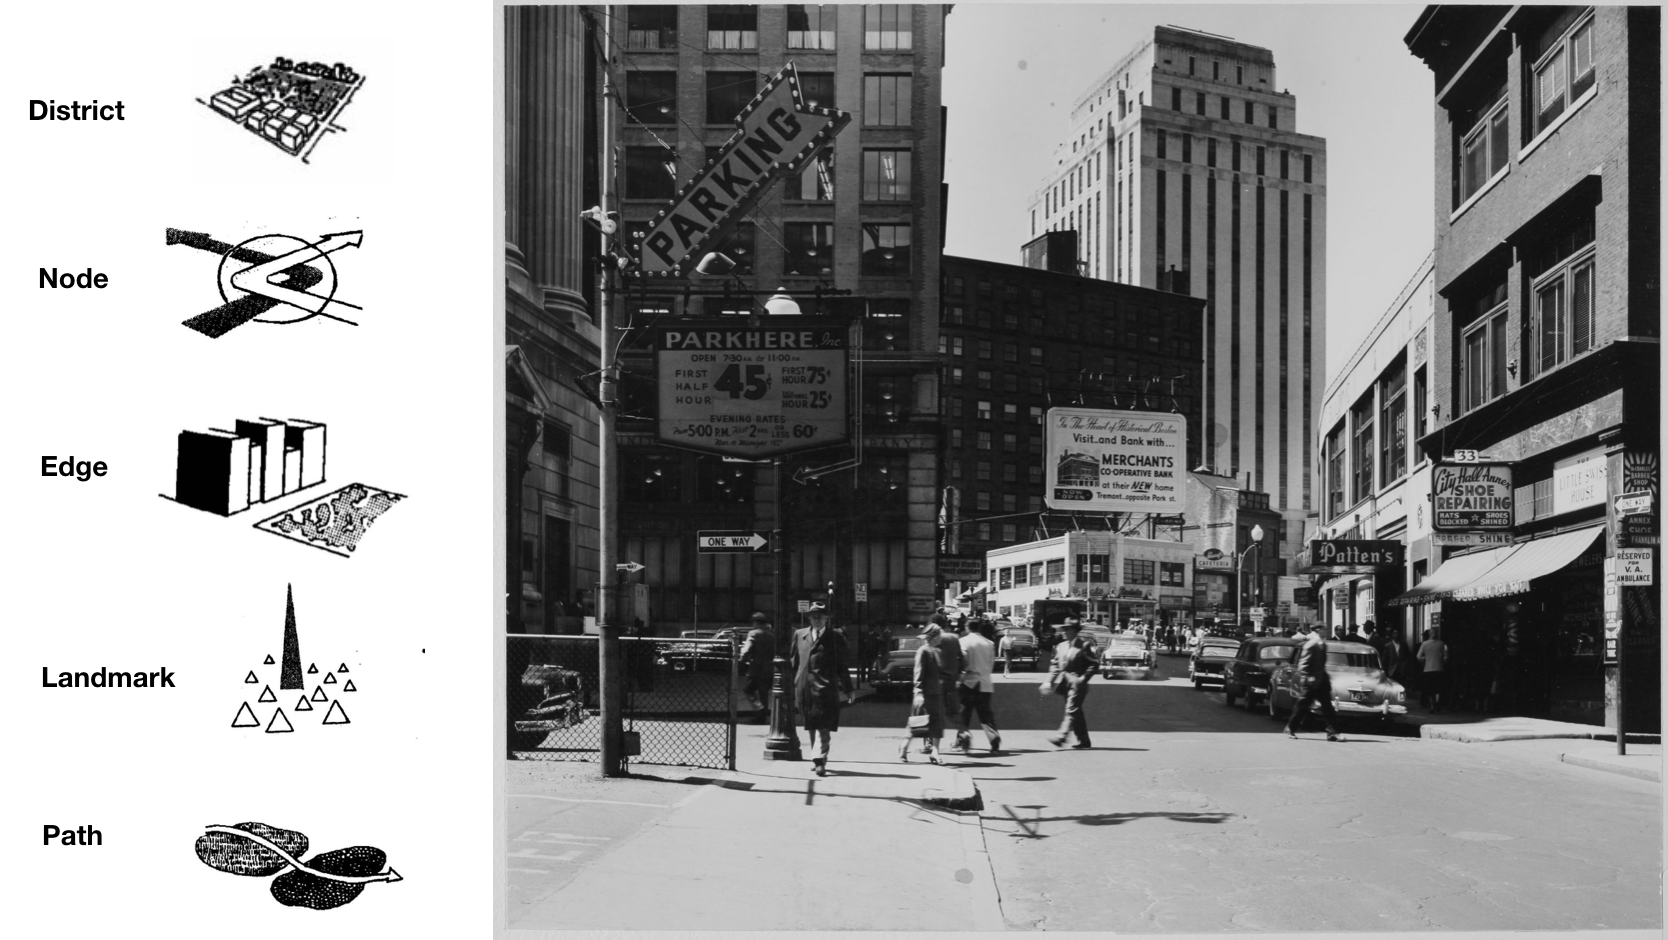
\includegraphics[width=1\columnwidth]{chapters/prediction/deepscope/figures/deepscope5.png}
                \caption{Urban `Imageability'. (left) Kevin Lynch's imageability classification metric for street element and urban experience. (right) An example street view, in which many of these classes are homogeneously interconnected \cite{lynch1960image}.}~\label{fig:deepscope_lynch}
            \end{figure}

            In 1960, MIT professor and Urbanist Kevin Lynch, introduced the idea of urban `imageability': a novel approach to visual perception of the built environments \cite{lynch1960image}. Lynch suggested a new classification of city-form, in which nodes, landmarks, paths, edges and districts reflect the sensation of traversing through the urban scape. Figure \eqref{fig:deepscope_lynch} demonstrates Lynch's imageability  and their manifestation in the streetscape. In the 1964 `The View From the Road' study \cite{appleyard1964view}, Lynch tested the idea of `imageability' using a new medium: He mounted a film camera to a car dashboard, and went on several day rides around five US metros \cite{Andrews2007}. When later played, these recordings were sped to reflect the overall `feel' of the urban skyline, overlooking nuanced street elements and architectural details, and prompting questions such as: What is the composition of the built mass? What shapes the street-section? Are there any noticeable landmarks, forms, or gaps? \cite{carr1969city, pearce1996legacy}.
        }

        \subsubsection{Urban Visualization}
        {
            Lynch's work contributed to the notion that street-level views are critical during initial urban-design stages, when the urban context is only being established \cite{drettakis2007design, brusaporci2017importance}. In the last few decades, advancements in computer graphics made it easier to visualize future urban developments \cite{shiode20003d, kempenaar2016design}. Nevertheless, few tools provide realistic and real-time urban visualizations, which can also be used as part of collaborative design processes \cite{mueller2018citizen}.
            \newline
            Most common visualization tools carry complex setups, costly hardware and software, as well as steep learning curves \cite{yan2014evaluation, mekni2014augmented}. These tools often require users to set up many control parameters, such as cameras, lights, and materials, and constantly adjust these to produce decent results. This process can become laborious in complex design scenes, and can gravely affect the outcome, cost and duration of visualization processes, and the design process as a whole \cite{lovett2015using}.
        }
    }


    \begin{figure}[!htb]
        \centering
        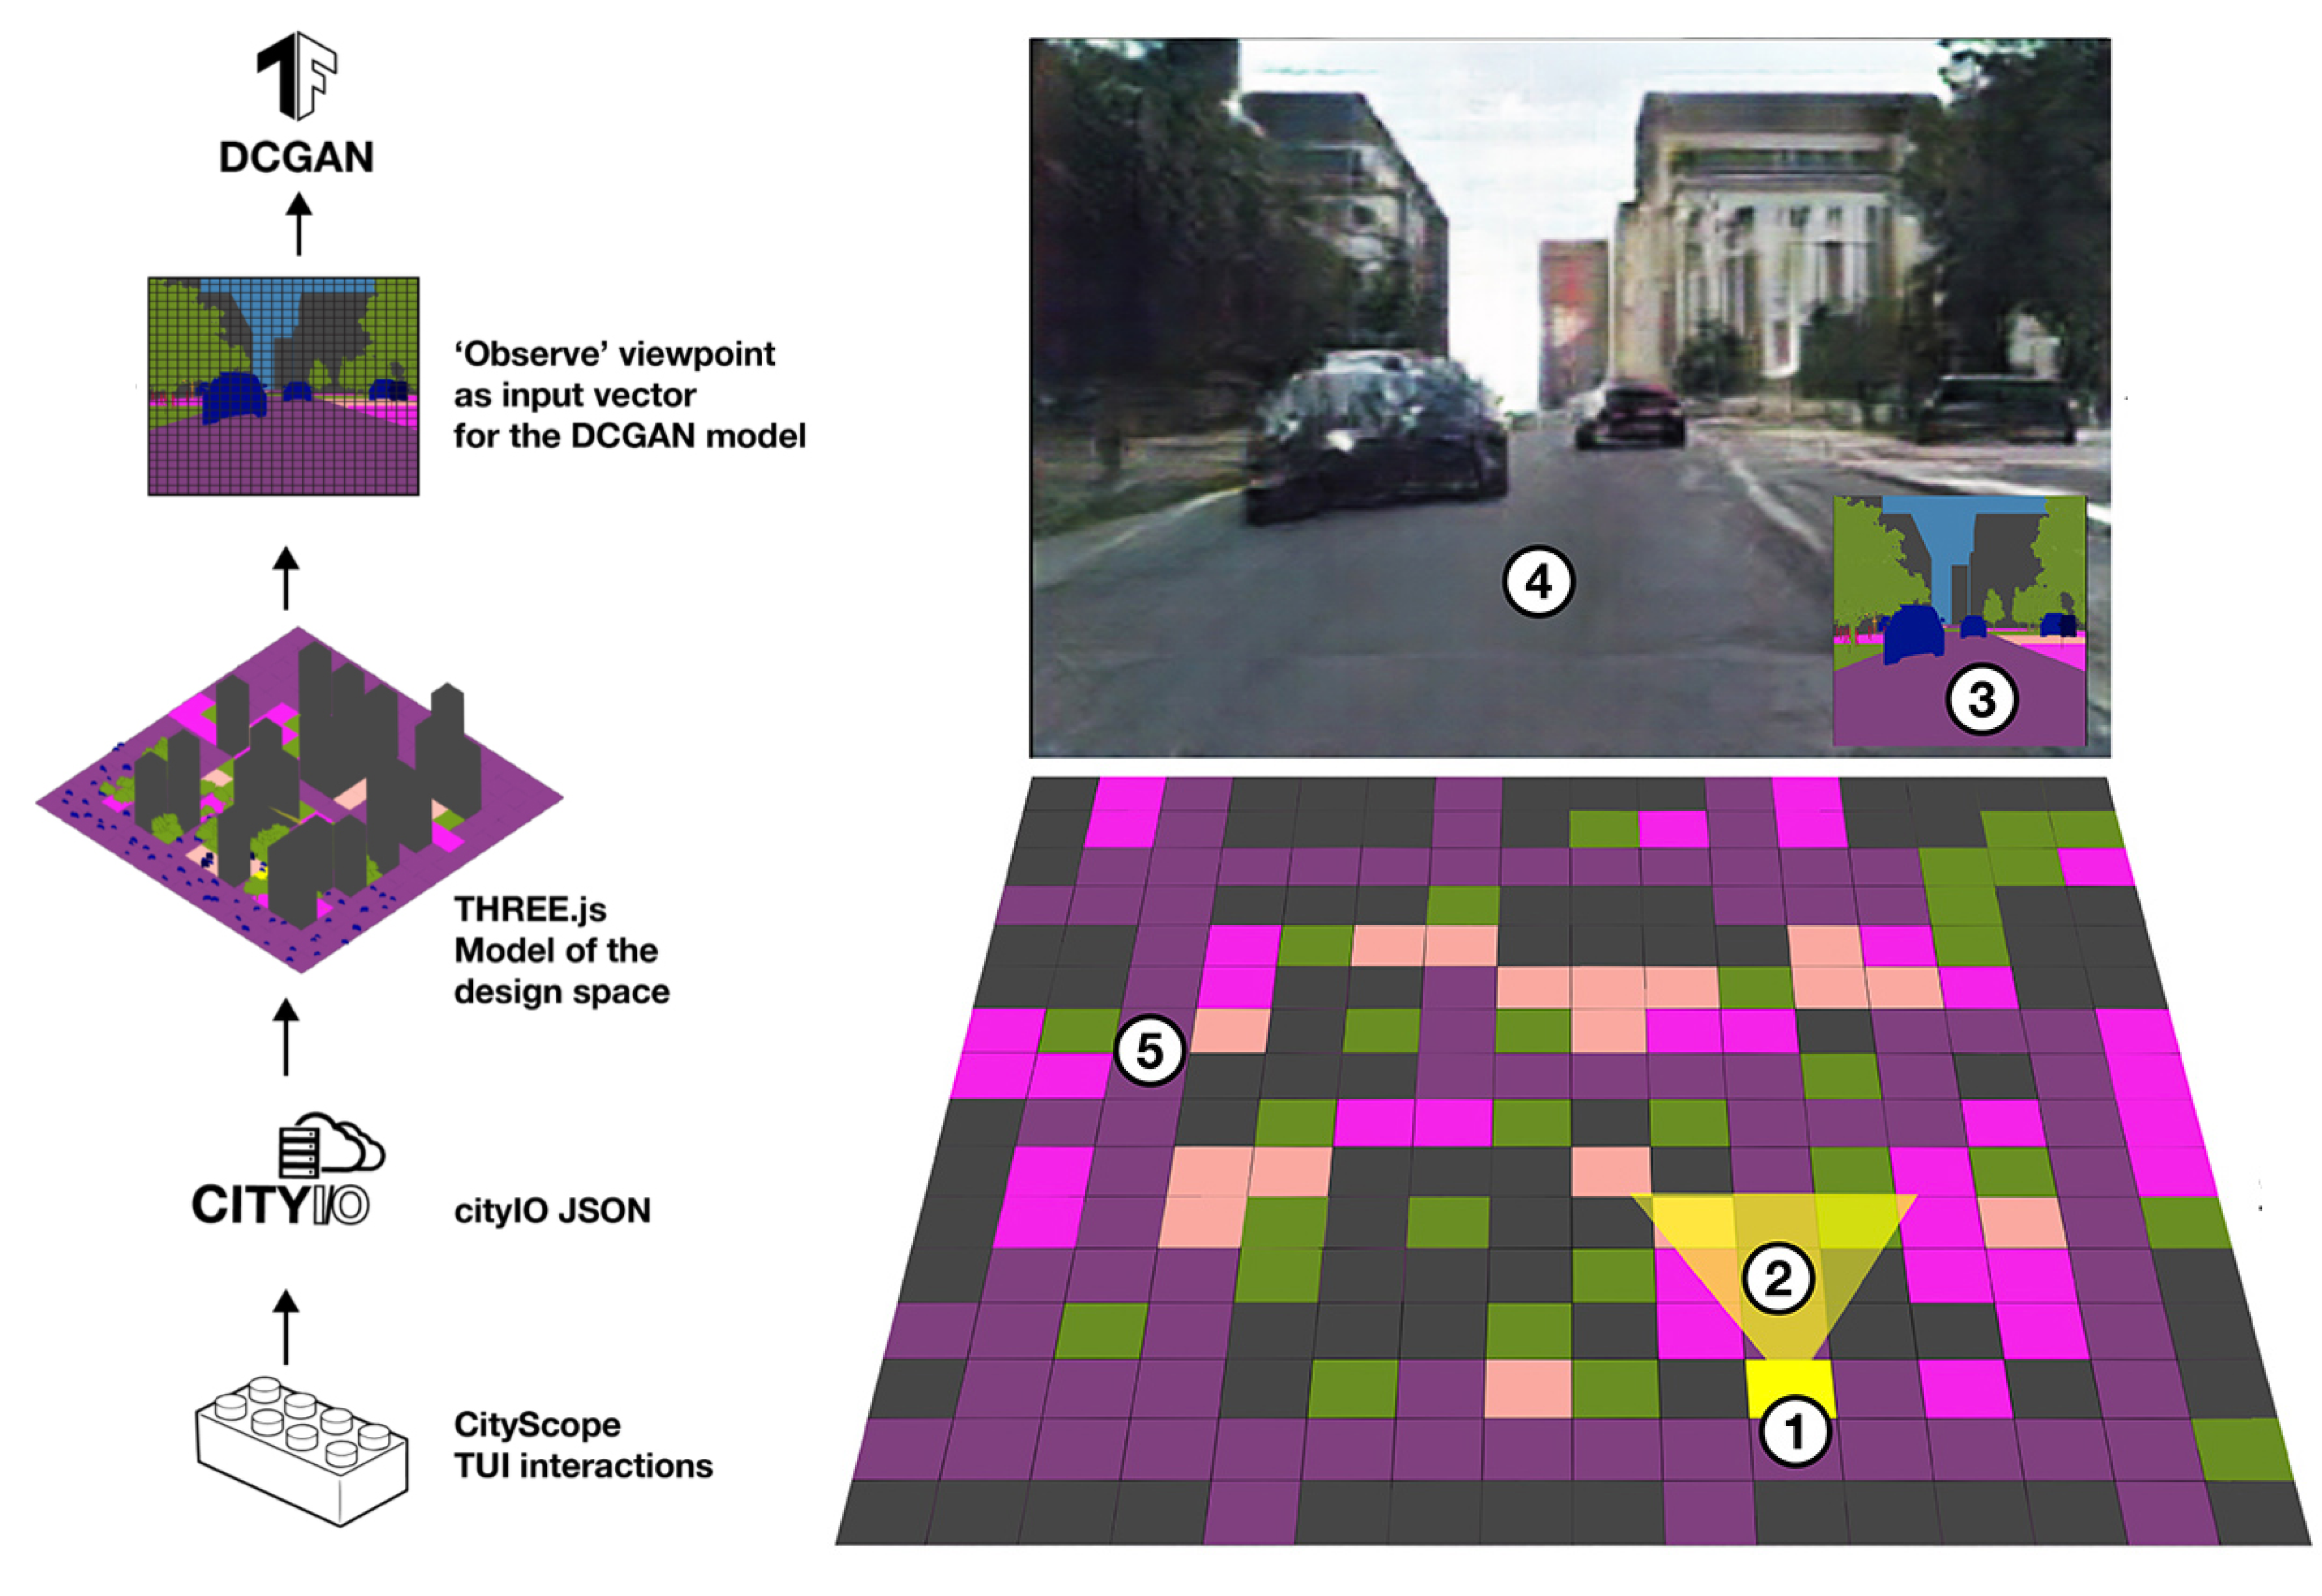
\includegraphics[width=1\columnwidth]{chapters/prediction/deepscope/figures/deepscope3.png}
        \caption{From interaction to prediction. (left) TUI interactions are captured using OpenCV and streamed to the webGL app. A 3D model is created based on the grid's JSON array and the Observer viewing angle. Lastly, a snapshot image is fed as an input vector to the DCGAN model. (right) (1) Observer position (2) Observer view angle and FOV cone (3) Observer's 3D street-view as input for DCGAN (4) DCGAN model prediction of street-view (5) TUI interactive grid.}~\label{fig:deepscope_dataflow}
    \end{figure}



    \subsection{System Design}\label{DeepScope-system-architecture}
    {
        DeepScope is a CityScope module for collaborative, tangible, and real-time urban-design visualization. DeepScope allows multiple users to collaboratively observe the visual outcomes of early planning stages using autogenerated visualizations. As with other CityScope platforms, DeepScope requires minimal setup, basic hardware and software, and no expertise to use\footnote{For general design of CityScope platforms see Section \eqref{sec:cityscope_architecture}}.

        \subsubsection{DeepScope User Interaction}\label{DeepScope-user-interaction}
        {
            DeepScope TUI is composed of three components: (i) A physical urban model, (ii) a scanning module, and (iii) a feedback module. The urban model includes an arbitrary grid of LEGO tiles, tagged with binary patterns, and scanned using CityScoPy as discussed in Section \eqref{subsec:csarch-cityscopy}. Figure \eqref{fig:deepscope_users} depicts a user positioning a tagged LEGO brick into the TUI design space to trigger the model generation.

            \begin{figure}[!htb]
                \centering
                \includegraphics[width=0.6\columnwidth]{chapters/prediction/deepscope/figures/deepscope2.png}
                \caption{
                    Multi-user interaction with DeepScope.
                    Multiple users can simultaneously interact and discuss urban-design iterations. The table-top is used as both the design space and a schematic urban top-view. The vertical monitor visualizes the DCGAN street view.
                }~\label{fig:deepscope_users}
            \end{figure}

            In DeepScope, each grid-cell pattern represents a different streetscape class, such as roads, buildings, green-spaces, parking, or sidewalks. Each class contains additional parameters, such as height, volume, shape, rotation and density. Table \eqref{deepscope:tab-types-classes} specifies the classes and their attributes.


            \begin{table}
                \begin{center}
                    \caption{
                        Cityscapes dataset classes used in DeepScope. Marked with `plus' are labels which can be altered dynamically using CS TUI. Marked with `star' are labels that are generated dynamically in the 3D model.
                    }
                    \label{deepscope:tab-types-classes}
                    \begin{tabular}{l|l}
                        \hline
                        \textbf{Group} & \textbf{Classes}                                                     \\
                        \hline
                        flat           & road*+; sidewalk*+ parking*+; rail track                             \\
                        human          & person*; rider*                                                      \\
                        vehicle        & car*; truck*; bus*; on rails; motorcycle; bicycle*; caravan; trailer \\
                        construction   & building; wall*; fence; guard rail; bridge                           \\
                        object         & pole*; pole group; traffic sign*; traffic light*                     \\
                        nature         & vegetation*+; terrain                                                \\
                        sky            & sky*                                                                 \\
                        void           & ground; dynamic; static
                    \end{tabular}
                \end{center}
            \end{table}
        }

        \subsubsection{Procedural Environment}
        {
            With each user interaction, the scanner decodes the array of grid-cell patterns and updates the CityScope Schema (see Section \eqref{sec:cityscope_architecture}). This triggers a generation of a virtual 3D environment, in which each grid-cell is represented via its class and additional parameters (see Figure
            \eqref{fig:deepscope_dataflow}
            ). As users allocate tiles, the 3D environment is procedurally populated with streetscape elements. For example, a vegetation pattern will create a surface with procedural trees, bushes or live-fences; A sidewalk pattern will produce pedestrians and street-signage, and a parking-lot pattern will be proliferated with parked vehicles. The generated 3D environment is uniformly hued with RGB values that correspond to input classes which correspond to the Cityscape dataset classes, and are expected by the GAN model (see Section \eqref{DeepScope-Generative-Model}). The 3D scene generation is done on the client-side web-browser using WebGL and ThreeJS \cite{mrdoob_2019}.
        }


        \begin{figure}[!htb]
            \centering
            \includegraphics[width=0.7\columnwidth]{chapters/prediction/deepscope/figures/deepscope4.png}
            \caption{DeepScope TUI. (top) TUI and the Observer tile. (left) User interaction with grid-cells. (right) `Observer' viewing angle, depth and position is set via an Arduino game-pad}~\label{fig:deepscope_observer}
        \end{figure}


        \subsubsection{Observer}\label{observer}
        {
            The urban environment designed by the users is constantly captured by the `Observer' grid-cell. Similar to Lynch's `View form the Road' \cite{appleyard1964view}, this one-off unique CityScoPy pattern, mimics a virtual nomad traversing through the city. The Observer allows users to sets the position, point-of-view and angle of a virtual camera in the 3D scene, so that real-time visualizations will be predicted from that view. The Observer baseline parameters (such as FOV, Frustum and camera-height) were approximated to the camera calibration appendix of the Cityscapes dataset used in model training \cite{Cordts2016}. Additional camera controls were implemented to allow users to move, rotate, pan or zoom the Observer via custom game-pad joystick (see Figure \eqref{fig:deepscope_observer}).
        }

        \subsubsection{Tabletop Feedback}\label{deepscope-table-top}
        {
            As with other CityScope instances, DeepScope tabletop is used as both the design space and a canvas for data visualization. With each design iteration, an illuminated land-use diagram is projected onto the table-top, so that each tile is showing its respective pattern, name or parameters (density, land-use, etc.). The Observer position is displayed using perspective cone that indicates its current viewing angle and FOV (see Figure \eqref{fig:deepscope_dataflow}).
        }
    }

    %%%%%%%%%%%%%%%%% GAN  %%%%%%%%%%%%%%%%%% 


    \begin{figure}[!htb]
        \centering
        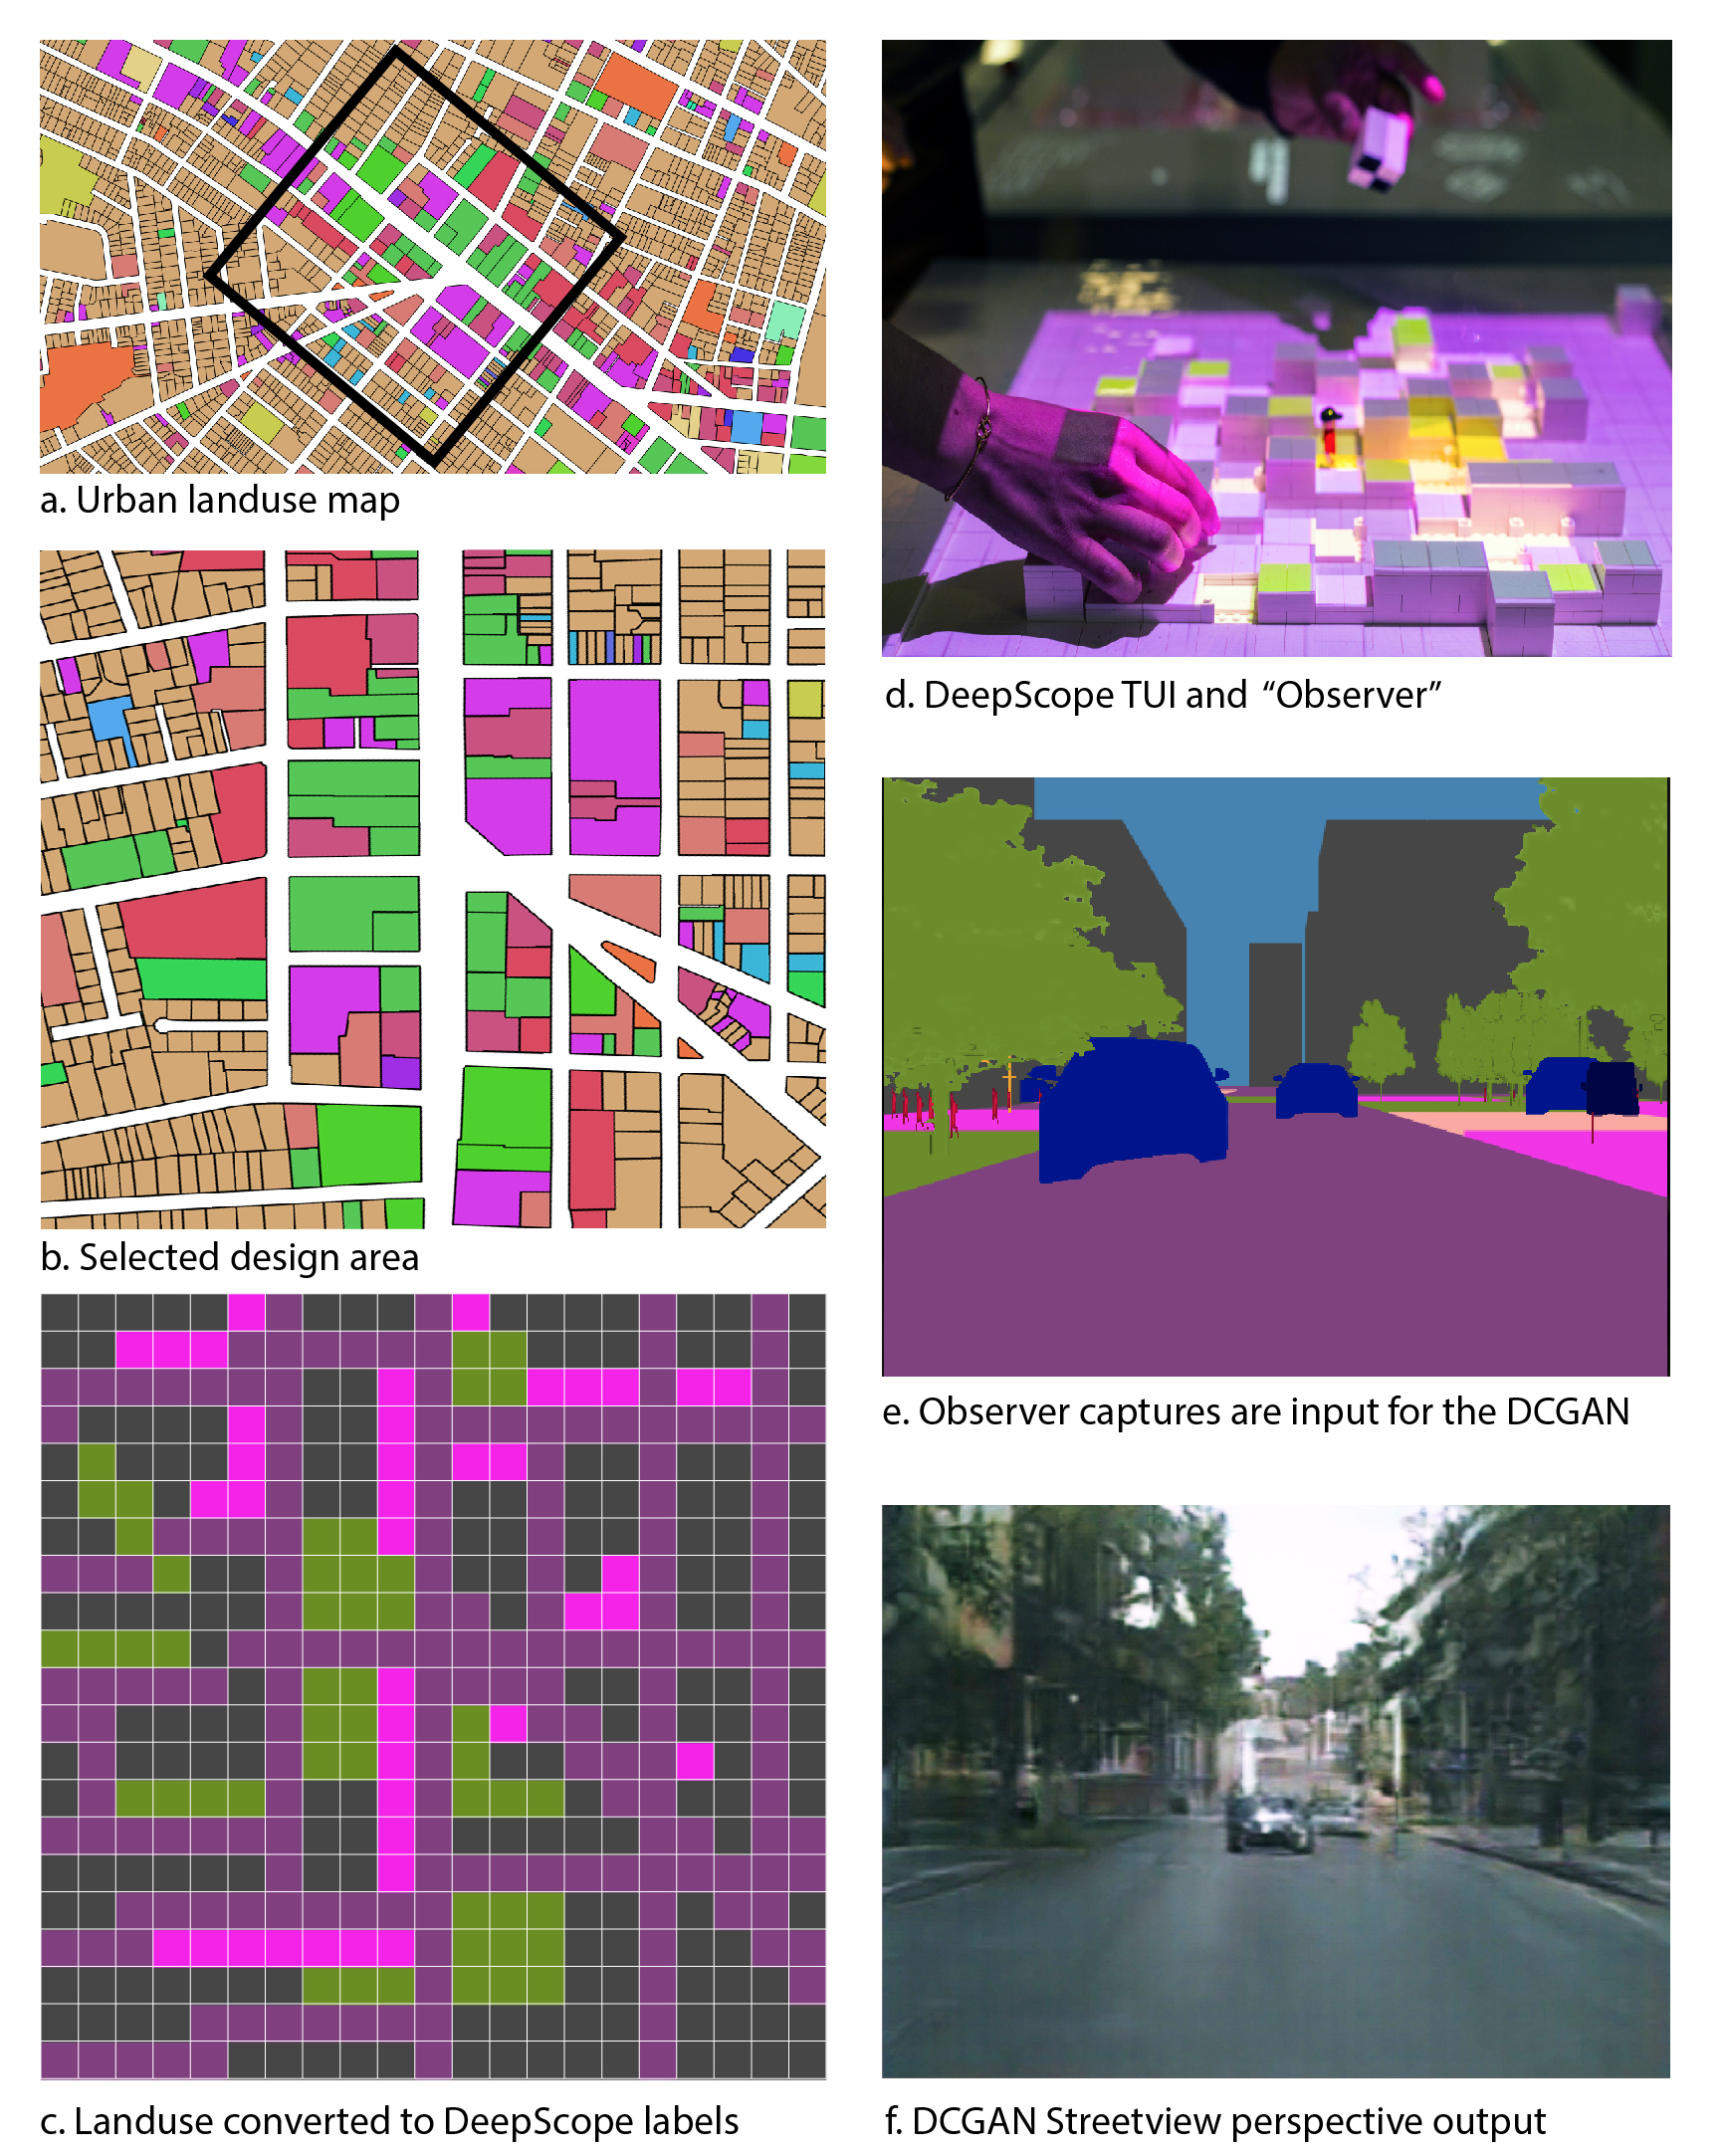
\includegraphics[width=0.5\columnwidth]{chapters/prediction/deepscope/figures/deepscope6.jpg}
        \caption{From site to prediction. This process depicts site selection, conversion to CityScope Schema, interaction, and prediction using the DCGAN model.}
        \label{fig:deepscope_pixelation}
    \end{figure}

    \subsection{Generative Model}\label{DeepScope-Generative-Model}

    {
        DeepScope uses a Deep Convolution Generative Adversarial Network (DCGAN) in order to generate street-view visualization in real-time. With each TUI interactions, the Observer viewpoint is captured as an input vector, used by the DCGAN model to predict an image (see Figure \eqref{fig:deepscope_dataflow}). The DCGAN generates an bitmap corresponding to the input vector, where each pixel in the input vector triggers the prediction of a corresponding pixel in the DCGAN output. The resulting image is then drawn onto the DeepScope feedback module.
    }

    \begin{figure}[!htb]
        \centering
        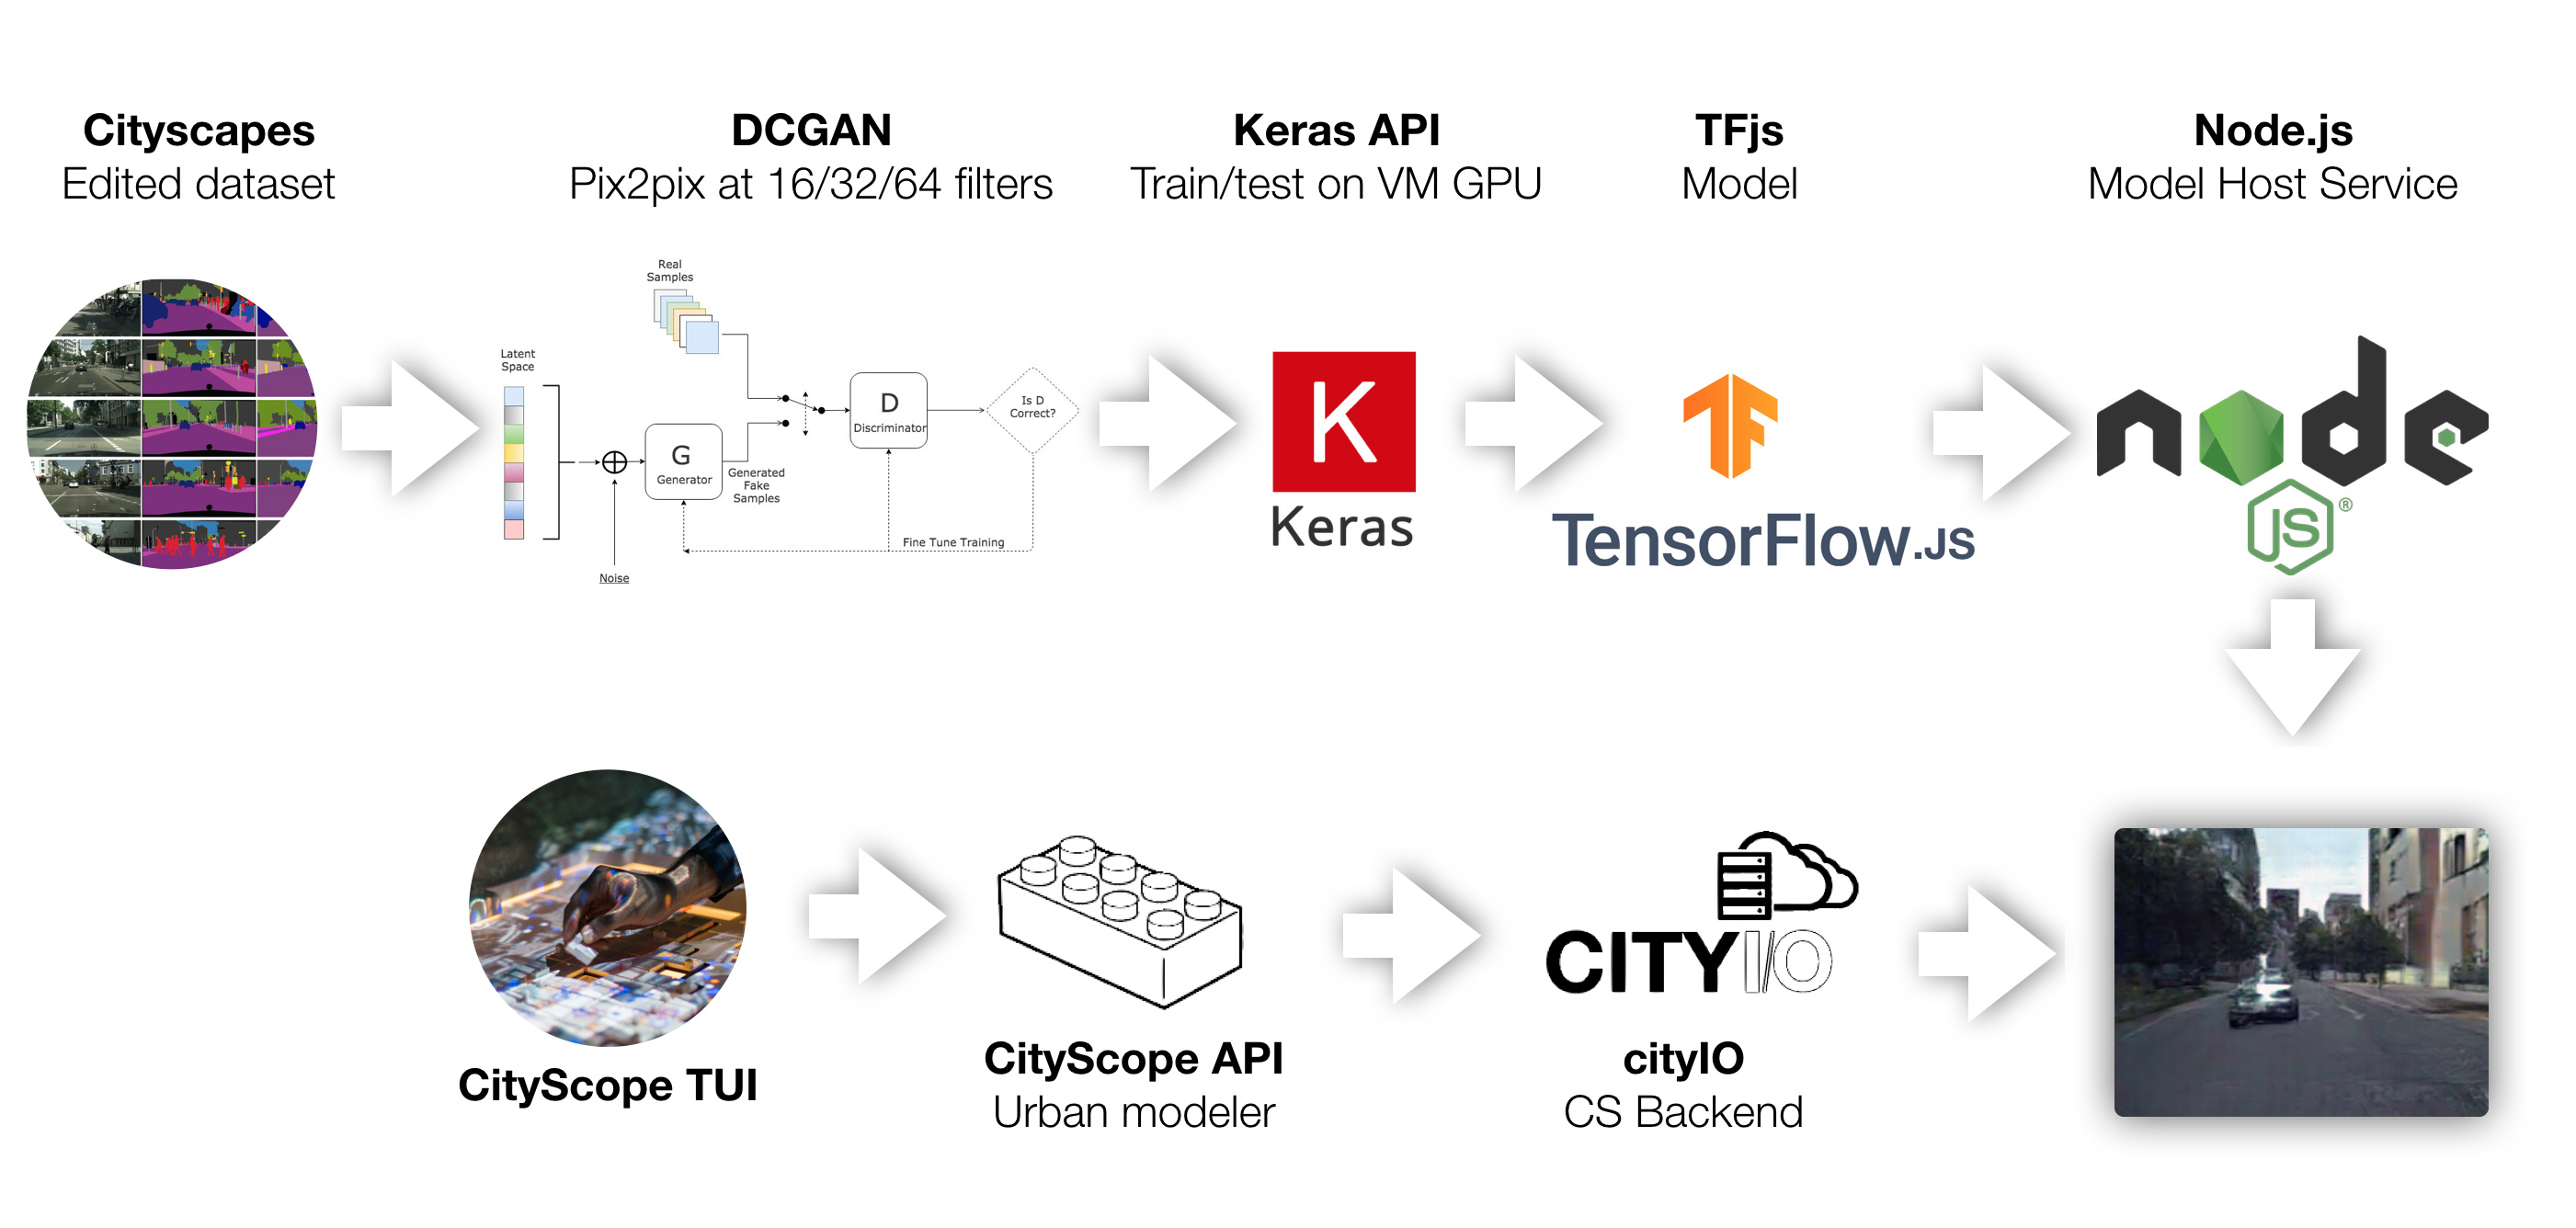
\includegraphics[width=1\textwidth]{chapters/prediction/deepscope/figures/deepscope0.jpg}\caption{(Top row) Model trained on Cityscapes dataset, deployed as node.js app. (Bottom row) TUI triggers DCGAN renderings.}~\label{fig:deepscope_arch}
    \end{figure}

    \subsubsection{Dataset and Model Training}\label{model-and-data}
    {
        Accurate pattern recognition using neural networks (NN) was already possible in the late 1980's \cite{lecun1989backpropagation}. However, generating new data that well concatenates a given dataset is still considered a complex problem in Machine Learning \cite{creswell2018generative}. Data generation using NN was greatly advanced with the introduction of Generative Adversarial Networks (GAN) \cite{Goodfellow2013}. GAN use two competing NN, a Generator and a Discriminator, that `adverse' one another; The Generator attempts to create new data (such as image, sound or text), and the Discriminator aims to nullify these data by comparing them to the distribution of a ground-truth data. The training is usually completed when the Generator can create close to indistinguishable samples which can fail the Discriminator \cite{pix2pix2016}.
    }


    \subsubsection{Image-to-Image Translation}\label{image-to-image-translation}

    {
        A variant of GAN is Conditional GAN (CGAN), in which both NN are given additional data that focuses the generation on specific targets \cite{mirza2014conditional, salimans2016improved}. A notable use-case of CGAN is a pixel-wise conditional generation of images, known as Image to Image Translation or `pix2pix' \cite{isola2017image, pix2pix2016}. In pix2pix, pairs of images are used for training, where the pixel values of one image are used as labels (also known as `classes') of the other. This allows pixel-level prediction using spatial classification of regions in the image \cite{arjovsky2017wasserstein, zhu2017unpaired}. In practice, CGAN extends the classic GAN zero-sum objective function with additional class data so that:
        \begin{equation} \label{deepscope-gan-objective-function}
            \min_G \max_D V(D, G) = \mathbb{E}_{\bm{x} \sim p_{\text{data}}(\bm{x})}[\log D(\bm{x} | \bm{y})] + \mathbb{E}_{\bm{z} \sim p_z(\bm{z})}[\log (1 - D(G(\bm{z} | \bm{y})))]
        \end{equation}
        where function ${V}$ of the Generator and the Discriminator ${G, D}$ attempts to minimize a delta between ground-truth data ${x}$ (in this case, the pixel data) and ${z}$, which is the accumulated pixel distribution learnt on each training step (see Figure \eqref{fig:deepscope_epoch}). Unlike classic GAN, $\log_{D(\bm{x} | \bm{y})}$ denotes that the additional `class' data ${y}$ conditions the learning on both data \textit{x} as well as on ${y}$ class. In this respect, CGAN generator do not only generate data with resemblance to the learnt distributions, but can closely mimic details in the data structure. DeepScope implements a variant of pix2pix that is fast and lightweight enough for real-time predictions in web browsers of low-tier devices.
    }


    \subsubsection{Cityscapes Dataset}\label{cityscapes-dataset}
    {
        The DeepScope DCGAN model was trained on the Cityscapes dataset \cite{Cordts2016}. Cityscapes is composed of pairs of street-view images taken using a dashcam around 50 European cities, during different seasons, daytime and weather conditions. Each pair includes a street-view image and a corresponding segmented image with 30 semantic labels (`classes'). These labels represent different streetscape classes, from buildings and roads to license-plates and road signs. For DeepScope, a pre-processing algorithm was designed to remove motion-blur, increase sharpness, saturation and remove color-casting, which were common in a shots taken by a moving vehicle. This pre-processing tools was built in Python OpenCV \cite{opencv_library}.

    }

    \subsubsection{Model Architecture and Performance}\label{dCgan-model-architecture-and-performance}
    {
        The model architecture of DeepScope was designed to allow fast predictions and portability for web-based devices. The Generator network has 16 layers with a U-Net encoder-decoder structure \cite{ronneberger2015u}. For performance purposes, the Discriminator has only 5 layers and is using Leaky ReLU activation that has been shown to improve stability in training \cite{Radford2015}. Commonly, DCGAN models benefit from higher number of filters \cite{ronneberger2015u}, however more filters also increase the model size, which can impact real-time performance and usability in low-tier devices. In order to still maintain attention to fine details, a shallow network design with a random up-sampling of 150\% was used \cite{isola2017image}. This network allows deployment on client-side browsers or mobile devices where TensorFlowJS is supported \cite{smilkov2019tensorflow}.
    }



    \begin{figure}[!htb]
        \centering
        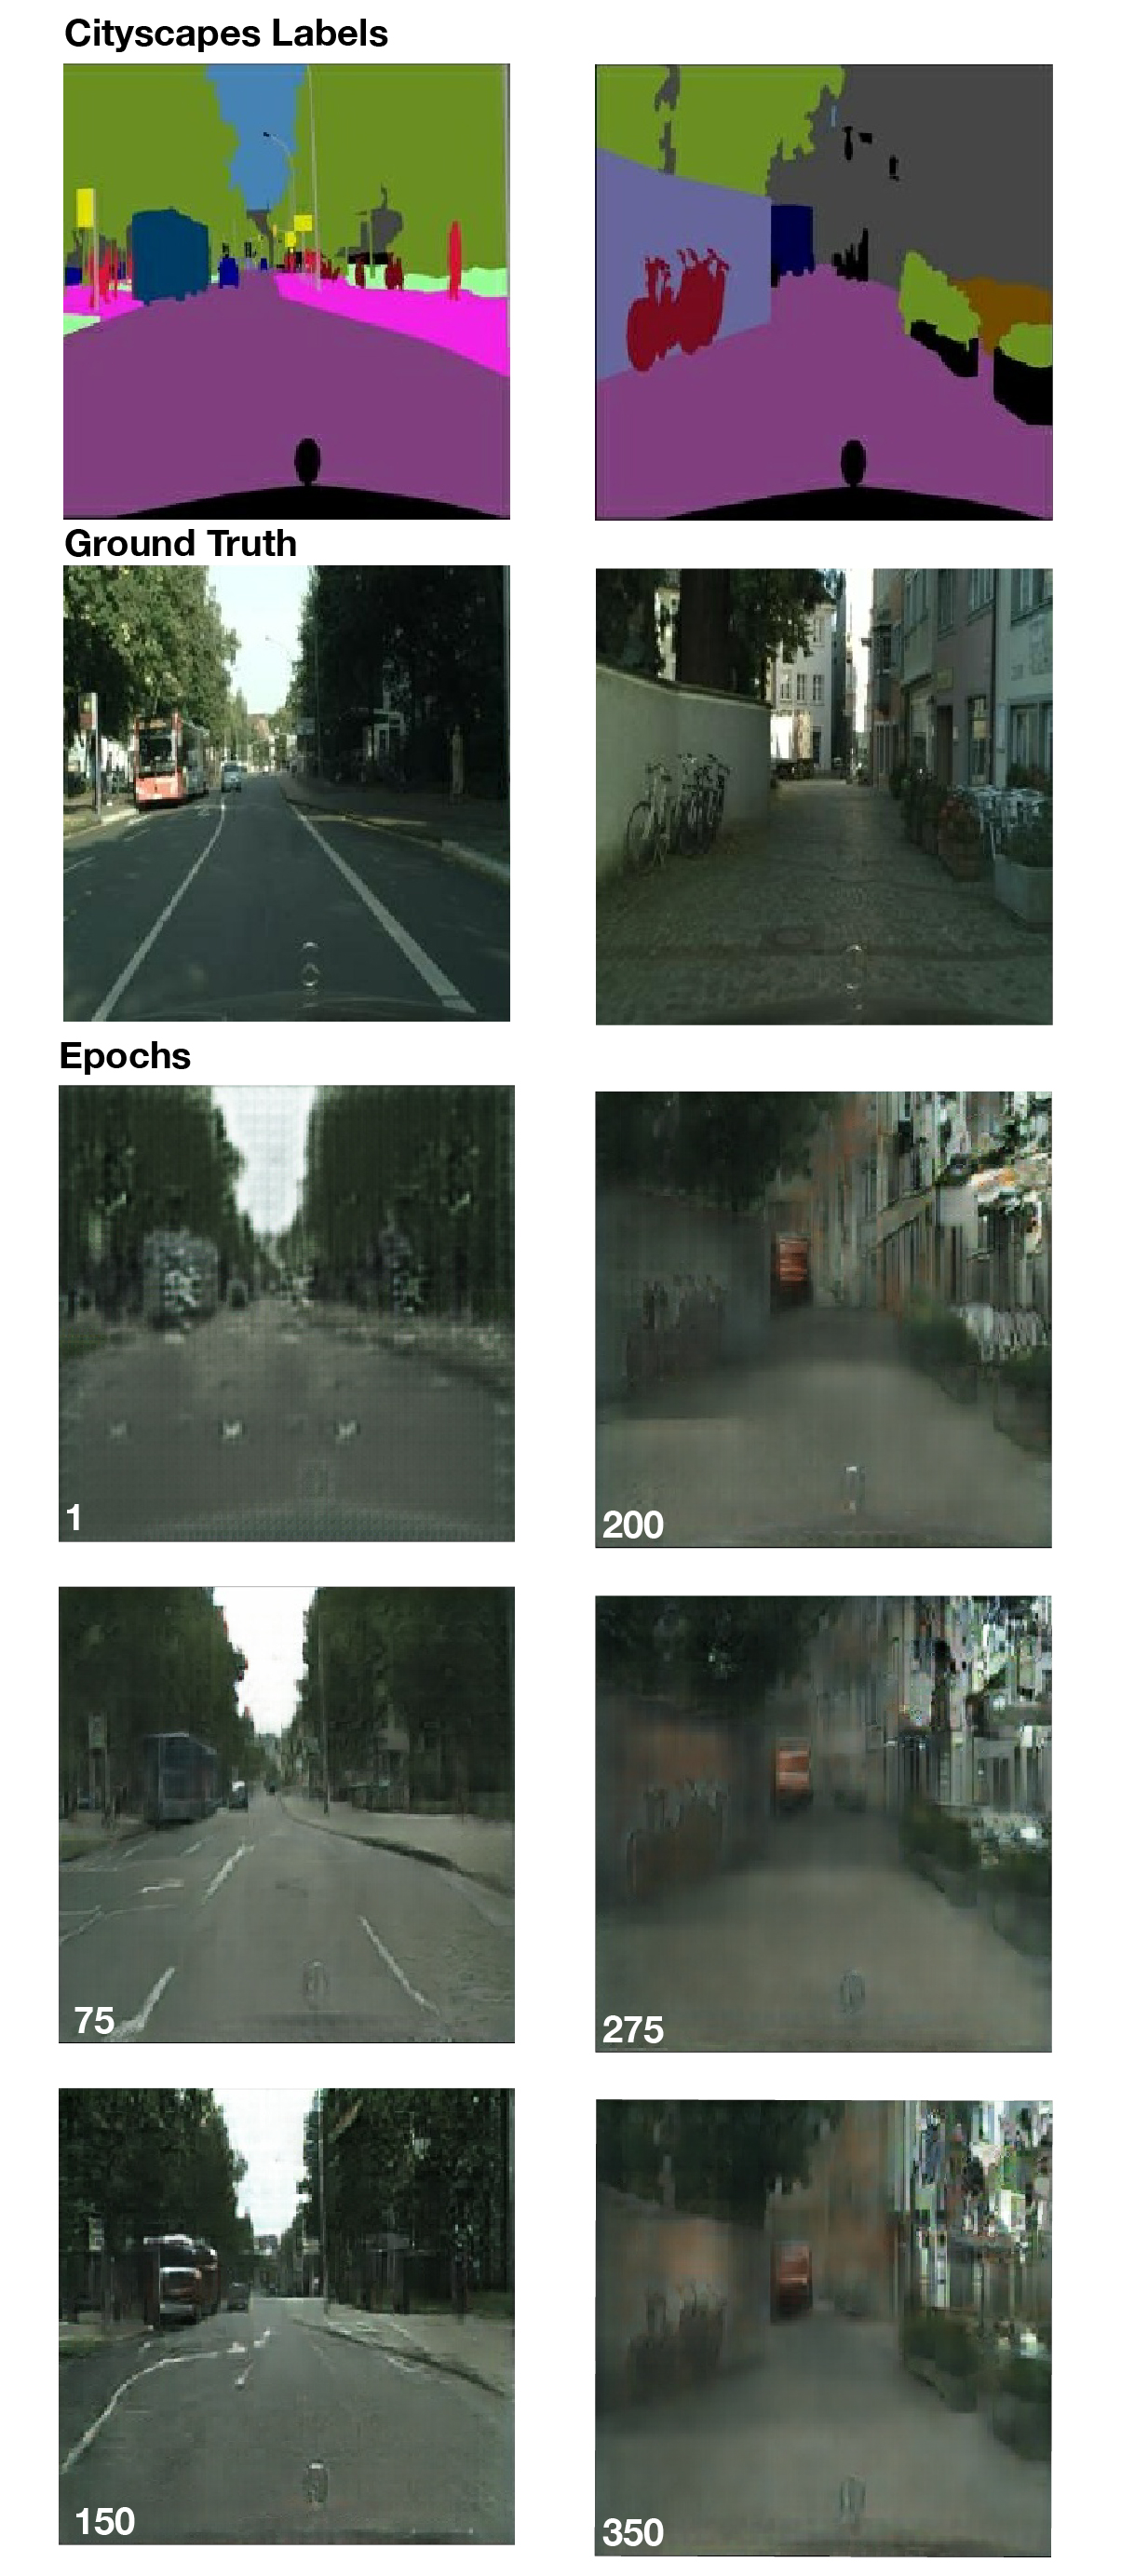
\includegraphics[width=0.3\columnwidth]{chapters/prediction/deepscope/figures/deepscope1.jpg}
        \caption{Test samples during training. Right column shows quality degradation beyond $\sim$200 epochs.}~\label{fig:deepscope_epoch}
    \end{figure}


    \subsubsection{DCGAN Training and Results}\label{dCgan-training-and-results}
    {
        20 training sessions were conducted with 16, 32, 64 and 128 filters, and 50 to 2000 epochs. Resulting models were converted to a \verb|JSON| format and tested for stability and response time on various browsers. A trained model with 64 filters and 200 epochs showed the best overall results. Models with less filters produced low-quality results; models with up to 2000 epochs demonstrated inconsistencies and `mode collapse' \cite{arjovsky2017wasserstein}.
    }


    \subsubsection{UI Performance Test}\label{deepscope-platform-and-user-interaction}
    {
        In order to avoid interaction latency, two asynchronous processes were used: (i) prediction process, and (ii) TUI interaction response. In user tests, the DCGAN model predicted at $0.66 sec/prediction$ on an average desktop system used by CityScope instances; the TUI has a fixed response interval of 50ms. Although DCGAN predictions slightly trails the TUI, the observation showed that users tend to focus their attention to the horizontal TUI before expecting the DCGAN output. Therefore, the overall user experience could be considered real-time with continuous design-and-feedback loops \cite{deber2015much}.
    }


    \subsection{Discussion}\label{deepscope-discussion}
    {
        DeepScope is a CityScope module which uses a real-time neural-network model to provide early stage urban-design visualization of skylines and streetscapes. Different from previously explored analysis modules, DeepScope aim is not to predict the impacts of urban intervention with respect to physical urban systems; Instead, DeepScope is meant to offer an implicit impression of the prospective development during the design process. Alongside mobility, energy, and other spatial-physical metrics, DeepScope can be used to `hallucinate' the impact of urban interventions, thus adding another way to evaluate urban transformation. The rest of this section discusses the strengths, weaknesses, threats and opportunities of this work.



        \subsubsection{Strengths}\label{strengths}
        {
            Early urban-design stages have major impacts on the spatial organization of cities, but commonly lack sufficient design representation and clear `image' \cite{Batty2000}. DeepScope is designed to allow experts and non-professionals alike to collaboratively experiment with urban-design scenarios and real-time feedback. The platform can augment early stages of urban-design with near real-life street-view visuals. The `unpolished' nature of the visualizations forces designers and regulators to focus on the overall `Image of the City', instead of highly-specific design details \cite{lynch1960image}. Unlike traditional tools, the complexity of creating a detailed urban scene is carried out by a lightweight, pre-trained neural network, which is triggered by an intuitive TUI.
        }

        \subsubsection{Weaknesses}\label{weaknesses}
        {
            Despite their promise, GAN have several drawbacks. First, they require large and properly labeled datasets. For example, creating a Cityscapes-like dataset for other geographies will involve significant efforts. Several emerging methods suggest decoupled \cite{zhu2017unpaired} and label-less learning \cite{lucic2019high}, which can simplify the labeling effort. Nevertheless, dataset collection and partial labeling would still be required. Moreover, GAN tend to be inconsistent during learning process, as explored in Subsection \nameref{dCgan-training-and-results} \cite{shin2017continual}. Lastly, the DeepScope GAN would not be able to visualize non-street view angles: Since the Cityscapes dataset was captured using a vehicle dashcam, only matching angles produce reasonable predictions \cite{salimans2016improved}. This issue is common in other supervised networks, and requires either non-supervised methods or more extensive datasets.
        }


        \subsubsection{Threats}\label{threats}
        {
            The rising popularity of GAN is attributed to their ability to `create'; Nevertheless, GAN tend to produce unpredictable results. When it comes to the design practice, certain degree of `creative freedom' might be desired, yet unpredicted tools might cause resentment or misleading impressions. For example, in DeepScope, the same street-view angle with the same urban-design setup can produce different visual results if ran twice. Additionally, NN are strictly bounded to their architecture and training data. Tempered network or adversarial datasets can greatly affect the outcomes of the model and inject bias into the results. With machine-learning tools becoming mainstream in the design industry, these concerns should be addressed by testing, validating and open-sourcing design tools, models and data.
        }


        \subsubsection{Opportunities}\label{opportunities}
        {
            DeepScope can be improved in several aspects: First, emerging network architectures and training parameters can improve the DCGAN results. Other methods, such as VAE or auto-GAN, can produce finer results with greater control \cite{mescheder2017adversarial}. As well, extending the training datasets to different urban environments could yield more versatile representations and geographical relevancy. Lastly, the TUI can be improved to include multi-scale environments and more finer-grained editing capability.
            \newline
            More broadly, DeepScope might hint to a future of insightful urban-design tools, spanning beyond digital rulers and drafting aids. Such tools would not only expedite tedious tasks, but might be able to leverage the power of advanced computation and become digital design `companions'.
        }
    }
}

    %%%%%%%%%%%%%%%%%%%%%%%%%%%%%%%%%%%%%%%%%%% 

    \section{Discussion}
     {
      This Chapter discussed ways by which CityScope modules can support decision-making through the modeling of implicit aspects of the built environments. It focused on the impacts of urban development on temporal observations, such as mobility, and human dynamics in general \eqref{sec:revurb}, \eqref{sec:cityscope-mocho}, as well as demonstrated how the visual perception of urban-design can augment early-stage planning \eqref{sec:deepscope}. Further work in this field calls for urban models that seamlessly converge explicit and implicit aspects of urban development, and that can be used to support decision-making in complex scenarios \cite{dubey2016deep, moro2021mobility}. Work done on large-scale sentiment analysis of urban dwellers, thorough participatory or passive sensing, can be used in concert with traditional urban models to support the assessment of transformation. The next chapter, \textit{Consensus}, bring many of the ideas and techniques discussed in the first three chapters into a community-driven, and collaborative urban process, demonstrating how CityScope supported real-world decision-making in complex urban scenarios.
     }
    %%%%%%%%%%%%%%%%%%%%%%%%%%%%%%%%%%%%%%%%%%% 
}

